\chapter{PTC power plant}
%The PTC power plant was simulation in the \enquote{CSP parabolic trough (physical)} model in SAM using the option \enquote{no financial model}. As before the input the EPW weather file from Section~\ref{Solar radiation} was used to specify the hourly atmospheric conditions. 
%Also for the simulation of the PTC was the LCOE calculated separately using again the simplified method which is documented in Appendix~\ref{ChapterLCOE} on Page \pageref{ChapterLCOE}.

A parabolic trough plant was simulated using the \enquote{CSP parabolic trough (physical)} model in SAM and the option \enquote{no financial model}. The EPW weather file (see Section~\ref{Solar radiation}) was used to specify the hourly atmospheric conditions. 
Levelised cost of electricity was calculated separately using the simplified method (see Appendix~\ref{ChapterLCOE}, page \pageref{ChapterLCOE}).

\section{Design  and simulation} \label{PTC power plant design  and simulation}
%This section describes in detail the input data of the PTC power plant simulation by there components, namely the  power cycle, solar collector, solar receiver, solar field and thermal energy storage (TES). After that the belonging financial parameter are defind.

%In order to reaching the goal of covering 90 \% of the scheduled production curve also the simulated PTC power plant used a variation of solar multiple and full load hours of TES. To covering the scheduled load the solar multiple was varied from 2 to 5.0 in steps of 5.0. This is significantly higher SM compared the simulated CR system was necessary to reach the \SI{90}{\percent} covering factor. As before with the simulation of the CR, the storage full load hours were varied from \si{8} to \SI{16}{h} in steps of \SI{2}{h}. The target of \SI{100}{MW} net capacity was reached with a gross capacity of \SI{120}{MW} with an estimated gross-to-net conversion of \SI{83}{\percent}. The comparatively high gross turbine output is nessasary for the high parasitic burden of the system. Table~\ref{tbl: PTC_OverallConfig} summarizes the simulated configurations.

To reach \SI{90}{\percent} coverage of the prescribed load curve, the simulated PTC plant employed variable solar multiple and full load hours of TES. The solar multiple was varied from \num{2} to \num{5.0} in steps of \num{5.0}. This significantly higher SM compared to the simulated CR system was necessary to reach \SI{90}{\percent} coverage. Storage full load hours were again varied from \si{8} to \SI{16}{h} in steps of \SI{2}{h}. The target of \SI{100}{MW} net capacity was reached with a gross capacity of \SI{120}{MW} with an estimated gross-to-net conversion of \SI{83}{\percent}. The comparatively high gross turbine output is necessary due to the high parasitic burden of the system. Table~\ref{tbl: PTC_OverallConfig} summarizes the simulated configurations.

\begin{table}[!h]  
  \centering
	\begin{tabular}{ p{4.0cm}  C{1.0cm}  C{0.3cm} C{0.3cm} C{0.3cm} C{0.3cm} C{0.3cm} |C{0.3cm}  C{0.3cm} C{0.3cm} C{0.3cm} C{0.3cm} } 
	\hline	
\textbf{Item} & \textbf{Unit} & \multicolumn{10}{c}{\textbf{Value}} \\ \hline \hline
Net turbine capacity & \si{\mega\wattel} & \multicolumn{10}{c}{\num{100}} \\
Gross turbine capacity & \si{\mega\wattel} & \multicolumn{10}{c}{\num{120}} \\ \hline
Solar multiple & - & \multicolumn{5}{c}{\num{2.0}} & \multicolumn{5}{c}{\num{2.5}} \\
TES capacity & h & \num{8} & \num{10} & \num{12} & \num{14} & \num{16} & \num{8} & \num{10} & \num{12} & \num{14} & \num{16} \\ \hline 
Solar multiple & - & \multicolumn{5}{c}{\num{3.0}} & \multicolumn{5}{c}{\num{3.5}} \\
TES capacity& h & \num{8} & \num{10} & \num{12} & \num{14} & \num{16} & \num{8} & \num{10} & \num{12} & \num{14} & \num{16} \\ \hline 
Solar multiple & - & \multicolumn{5}{c}{\num{4.0}} & \multicolumn{5}{c}{\num{4.5}} \\
TES capacity& h & \num{8} & \num{10} & \num{12} & \num{14} & \num{16} & \num{8} & \num{10} & \num{12} & \num{14} & \num{16} \\ \hline 
Solar multiple & - & \multicolumn{5}{c}{\num{5.0}} & \multicolumn{5}{c}{ } \\
TES capacity& h & \num{8} & \num{10} & \num{12} & \num{14} & \num{16} &  \multicolumn{5}{c}{ } \\ \hline 
\end{tabular}
\caption[Simulated PTC solar multiple and thermal energy storage  configurations.]{Simulated PTC solar multiple and thermal energy storage  configurations.}\label{tbl: PTC_OverallConfig}
\end{table}

\subsubsection{Power cycle}
%The PTC system also uses the steam Rankine cycle technology. In the modeled cycle, feedwater is heated in open (mixed stream) feedwater heaters with two intermediate turbine extractions - once for high pressure and once for low pressure, and the steam generation equipment consists of a preheater, boiler, and superheater. The HTF temperature at the field outlet is bound primarily by HTF stability, so maximum HTF temperatures for oil troughs typically range between \SI{370}{\celsius} and \SI{410}{\celsius}. The turbine has a gross capacity of \SI{120}{\mega\wattel}. So the net turbine capacity output at design (nameplate) is \SI{100}{\mega\wattel}. The design inlet temperature of the HTF in the steam generator is 393\si{\celsius} and outlet temperature of 293\si{\celsius} at design point and operates at a pressure of 100 bar.

The PTC system also uses steam Rankine-cycle technology. In the modelled cycle, feedwater is heated in open (mixed stream) feedwater heaters with two intermediate turbine extractions - once for high pressure and once for low pressure, and the steam generation equipment consists of a preheater, boiler, and superheater. The HTF temperature at the field outlet is limited primarily by HTF stability, so maximum HTF temperatures for oil troughs typically range between \SI{370}{\celsius} and \SI{410}{\celsius}. The turbine has a gross capacity of \SI{120}{\mega\wattel}, so net turbine capacity output at its design point is \SI{100}{\mega\wattel}. The design inlet temperature of the HTF in the steam generator is \SI{393}{\celsius} and outlet temperature of \SI{293}{\celsius} at design point and operates at a pressure of \SI{100}{\bar}.

%Table~\ref{tbl: PTCPowerplant} shows the input parameter for the power block design in SAM. Besides the capacity of the turbine and the condecer type, the parameters are coming from \cite{Wagner2011}. It is obviously, that the cycle conversion efficiency of the PTC power plant is lower than that one from the CR power plant. This is trace back to the lower cycle temperatures and the thereby resulting lower steam pressure in the turbine.
Table~\ref{tbl: PTCPowerplant} shows the parameters for the power block design in SAM. All parameters except turbine capacity and condenser type are taken from \cite{Wagner2011}. Cycle conversion efficiency of the PTC power plant is lower than that of the CR power plant because of the lower cycle temperatures and the lower turbine steam pressure that results.

%It is not obviously :) (Nothing is obviously ;-) -- things are obvious, or obviously wrong. Obvious = Adjektiv, obviously = adverb



%The air-cooled condenser was selected here as well, because water is an valuable resource in the region of Upington. The cooling system is designed to covers the stem generator thermal power. 
The air-cooled condenser was selected, since water is scarce in the region. The cooling system is sized to dissipate the steam generator thermal power. 

\begin{table}[!h]  
  \centering
	\begin{tabular}{  p{7.0cm}  C{2.0cm}  C{2.0cm} } 
	\hline	
\textbf{Item} & \textbf{Value} & \textbf{Unit} \\ \hline \hline
Turbine design capacity, gross  & 110 & \si{\mega\wattel} \\ 
Turbine design capacity, net & 100 & \si{\mega\wattel} \\ 
Boiler operating pressure & 100 & bar \\ 
Design inlet temperature & 393 & \si{\celsius} \\ 
Design outlet temperature & 291 & \si{\celsius} \\ 
Cycle conversion efficiency & 37.74 & \% \\ 
Steam generator design thermal power & 318.0 & \si{\mega\wattth}  \\
Power block start-up time & 0.5 & h \\ 
Minimum required start-up temperature & 300 & \si{\celsius} \\
Maximum turbine over design operation & 90 & \\
Condenser type & air-cooled & - \\ 
\hline
\end{tabular}
\caption[PTC power block and condecer input parameters in SAM.]{PTC power block and condenser input parameters in SAM.}\label{tbl: PTCPowerplant}
\end{table}
\subsubsection{Solar collector (SCA)}
%For the simulation of the PTC system the Ultimate Trough was selected as solar collector assembly (SCA). This collector is currently not in commercial use, but comparable troughs with similar characteristics are under construction. So the Ultimate Trough can be adopted without technical modifications and no increase of risk. The technical input parameter of the Ultimate Trough for SAM coming directly from the developer (Flabeg GmbH and sbp sonne GmbH) and are documented in Appendix~\ref{PTCdocumentary} on Page~\pageref{PTC_Ultimate_config}. \cite{Riffelmann2014}

The Ultimate Trough was selected as solar collector assembly (SCA). This collector is currently not in commercial use, but comparable troughs with similar characteristics are being manufactured, so it is a reasonable choice and may be adopted without technical modifications or increased risk \cite{Riffelmann2014}. (For specifications, see Appendix~\ref{PTCdocumentary}, page~\pageref{PTC_Ultimate_config}.)


\subsubsection{Solar receiver (HCE)}
%As heat collecting element (HCE) Schott's PTR80 was selected. This receiver tube has with \SI{0.08}{m} an extended tube outer diameter. Thereby the tube can contain more HTF and reduce the mass flow in the tubes. The input data of the HCE for SAM comming from researchers of the American National Renewable Energy Laboratory (NREL) \cite{Kutscher2012}. The specified input parameter are documented in Appendix~\ref{PTCdocumentary} on Page~\pageref{PTC_HCE}. The total weighted losses of the HCE elements is \SI{207.35}{W/m} heat loss at design combined with about 0.85 optical derate (reduction in optical efficiency).
For the heat collecting element, Schott's PTR80 was selected. This receiver tube has an extended tube outer diameter of \SI{0.08}{m} to reduce flow velocity.

%The input data of the HCE for SAM comming from researchers of the American National Renewable Energy Laboratory (NREL) \cite{Kutscher2012}. The specified input parameter are documented in Appendix~\ref{PTCdocumentary} on Page~\pageref{PTC_HCE}. The total weighted losses of the HCE elements is \SI{207.35}{W/m} heat loss at design combined with about 0.85 optical derate (reduction in optical efficiency).

The specifications for the HCE in SAM are provided by the National Renewable Energy Laboratory (NREL) \cite{Kutscher2012}. The specific parameters used are documented in Appendix~\ref{PTCdocumentary}, page~\pageref{PTC_HCE}. The total weighted loss through the HCE elements is \SI{207.35}{W/m} heat loss at design point combined with about 0.85 optical derate (reduction in optical efficiency).


\subsubsection{Solar field}
%PTC solar fields are separated in sections. In the simulation of the PTC system the solar field is designed in two sections. Each section carries a feed pipe and a return pipe to transport the thermal energy to the power block. Attached to the header pipes are many loops, which contains the SCAs, the HCEs and the HTF. 

PTC solar fields are divided into sections. In the simulated system, the solar field has two sections. Each section carries a feed pipe and a return pipe to transport the thermal energy to the power block. Attached to the header pipes are many loops, which contain the SCAs, the HCEs and the HTF. 

%As mentioned before synthetic oil is used as HTF for the simulation of the PTC system, more precisely Terminol VP-1, which is currently the standard for HTF in PTC systems. Thereby is the system limited by the performance characteristics of Terminol VP-1 of 12 to 400\si{\celsius} \cite{Therminol2015}. The velocity range of Therminol VP-1 should be in the range of 0.36 and 4.97 m/s \cite{Wagner2014} and is affected by the inner tube diameter of the HCE, the HTF density and the loop flow rate \cite{NREL2015a}. A freeze protection temperature for the HTF of 150\si{\celsius} is typically and also assumed for the simulation \cite{Kearney2002}. The input parameter of the HTF for the PTC system are documented in Appendix~\ref{PTCdocumentary} on Page~\pageref{PTC_HTF}. 
A synthetic oil, Therminol VP-1, is used as HTF in this simulation. This limits the temperature envelope to \SIrange{12}{400}{\celsius} \cite{Therminol2015}. The velocity envelope of Therminol VP-1 is \SIrange{0.36}{4.97}{\meter\per\second} \cite{Wagner2014}. Actual stream velocity is determine by the inner tube diameter of the HCE, the HTF density and the loop flow rate \cite{NREL2015a}. (For the specifications of the HTF for the PTC system, see Appendix~\ref{PTCdocumentary}, page~\pageref{PTC_HTF}.) 

%The size of the solar field is strongly effected by the solar multiple and the thermal demand of the power block. At a solar multiple of \si{1} (design thermal power of the steam generator) the solar field requires \SI{453003}{\square\metre} ($\approx$\SI{45.3}{ha}) reflective aperture area of SCA. \si{65.86} ($\approx$66) loops are required at a SM of \si{1}. The number of loops and so also the field size multiplies by the value of the SM.
The size of the solar field is coupled to the solar multiple and the thermal demand of the power block. At a solar multiple of \si{1} (design thermal power of the steam generator) the solar field has \SI{453003}{\square\metre} (\SI{45.3}{ha}) of reflective aperture, corresponding to \si{65.86} ($\approx$66) loops.

%Also the the solar field area and thereby the total land area depending by the SM. Equation~\ref{GL_PTCSolarfieldarea} shows the influence on the solar field area of the ratio between the row spacing and the SCA width. The roe spacing is assumed by \SI{18}{m} between the parallel SCAs. The total land area results by Equation~\ref{GL_PTCtotallandarea} and is the solar field area multiplies by the factor of non-solar field area. The factor is assumed by \si{1.4} in the simulation \cite{NREL2015a}.

Equation~\ref{GL_PTCSolarfieldarea} shows the effect of row spacing to SCA width ratio on solar field area. The row spacing is assumed to be \SI{18}{m} between the parallel SCAs. The total land area is defined by Equation~\ref{GL_PTCtotallandarea} and is the solar field area multiplied by the factor of non-solar field area. A factor of \si{1.4} is assumed \cite{NREL2015a}.

\begin{align}
\textrm{solar field area }(m^2) =\textrm{aperture area }(m^2) \times \frac{\textrm{row spacing }(m)}{ \textrm{SCA width }(m)} \label{GL_PTCSolarfieldarea}
\end{align}
\begin{align}
\textrm{total land area }(m^2) =\textrm{solar field area }(m^2) \times  \textrm{non-solar field multiplier}\label{GL_PTCtotallandarea}
\end{align}
%Table~\ref{tbl: PTCSolarfield} shows the solar field simulation parameter of the PTC system for the simulation configuration values of the solar multiple. The parameters of the Table comes from the above mentioned relations between the Items. The design power of the steam generator (SG) stays at \SI{318.0}{\mega\wattth} while the solar field thermal output rises proportional through the SM. 
Table~\ref{tbl: PTCSolarfield} shows the solar field parameters of the PTC system for tested variations of the solar multiple. The parameters of the Table are determined from the relations given above. The design power of the steam generator (SG) stays at \SI{318.0}{\mega\wattth} while the solar field thermal output rises proportionally with SM. 

\begin{table}[!h]  
  \centering
	\begin{tabular}{ p{3.3cm} C{1.1cm} C{1.1cm} C{1.1cm} C{1.1cm} C{1.1cm} C{1.1cm} C{1.1cm} C{1.1cm} } 
	\hline	
\textbf{Item} & \textbf{Unit} & \multicolumn{7}{c}{\textbf{Value}} \\ \hline \hline
SG Design power & \si{\mega\wattth} &  \multicolumn{7}{c}{\num{318.0}}\\
Design-point DNI & \si{\watt\per\metre} &  \multicolumn{7}{c}{\num{950}}\\
\hline
\textbf{Solar multiple} &  & \textbf{2.0} & \textbf{2.5} & \textbf{3.0} & \textbf{3.5} & \textbf{4.0} & \textbf{4.5} & \textbf{5.0}\\ \hline 
Field thermal output & \si{\mega\wattth} & \num{636} & \num{795} & \num{954} & \num{1113} & \num{1272} & \num{1431} & \num{1590}\\
Number of loops  & - & \num{132} & \num{165} & \num{198} & \num{231} & \num{264} & \num{297} & \num{330}\\ 
Aperture reflective area & \si{\ha} & \num{90.6} & \num{113.3} & \num{135.9} & \num{158.6} & \num{181.2} & \num{203.9} & \num{226.5}\\ 
Total land area & ha & \num{675} & \num{845} & \num{1013} & \num{1182} & \num{1351} & \num{1540} & \num{1689}\\ 
\hline
\end{tabular}
\caption[PTC solar field parameters.]{PTC solar field parameters.}\label{tbl: PTCSolarfield}
\end{table}
\pagebreak
\subsubsection{Thermal energy storage (TES)}
%The thermal energy storage (TES) of the simulated PTC system uses a indirect two-tank molten salt system with "Hitec Solar Salt" as storage fluid. This storage fluid is made from sodium nitrate (60~\% NaNO\textsubscript{3}) and potassium nitrate (40~\% KNO\textsubscript{3}). Solar Salt needs an minimum operating temperature of 238\si{\celsius} and and has a maximum operating temperature of 593\si{\celsius}. \cite{Suite2011,Kearney2003}

The thermal energy storage (TES) of the simulated PTC system uses an indirect two-tank molten salt system with "Hitec Solar Salt" as storage fluid. This storage fluid is made from sodium nitrate (\SI{60}{\percent} NaNO\textsubscript{3}) and potassium nitrate (\SI{40}{\percent} KNO\textsubscript{3}). Solar Salt has a minimum operating temperature of \SI{238}{\celsius} and a maximum operating temperature of \SI{593}{\celsius} \cite{Suite2011,Kearney2003}.


\begin{table}[htbp]  
  \centering
	\begin{tabular}{ p{3.9cm}  C{1.0cm} C{1.2cm} C{1.2cm} C{1.2cm} C{1.2cm} C{1.2cm} } 
	\hline	
\textbf{Item} & \textbf{Unit} & \multicolumn{5}{c}{\textbf{Value}} \\ \hline \hline
Storage type & - &  \multicolumn{5}{c}{indirect two-tank molten salt}\\
Storage fluid & - &  \multicolumn{5}{c}{Hitec Solar Salt}\\
Hot tank design temp. & \si{\celsius} & \multicolumn{5}{c}{\num{391}}\\
Cold tank design temp. & \si{\celsius} & \multicolumn{5}{c}{\num{293}}\\
\hline
\textbf{TES full load hours} & \textbf{h} & \textbf{8} & \textbf{10} & \textbf{12} & \textbf{14} & \textbf{16}\\ \hline 
Thermal capacity & \si{\mega\wattth\hour}  & \num{2544} & \num{3180} & \num{3816} & \num{4452} & \num{5087} \\
Storage volume  & \si{\cubed\metre} & \num{34407} & \num{43008} & \num{51610} & \num{60212} & \num{68813}\\
\hline
\end{tabular}
\caption[PTC system TES parameter.]{PTC system TES parameter.}\label{tbl: PTCTES}
\end{table}

%The storage design temperatures depends from the solar field design temperatures, so the designed temperature difference is \SI{98}{K}. As it is shown in Table~\ref{tbl: PTCTES} the operating temperature limits fits with the storage tank design temperatures. The heater set point is 265\si{\celsius} for both storage tanks. The TES full load hours goes from 8 to 16 in steps of 2. The thermal capacity and also the storage volume rises with the TES full load hours. The simulated stored thermal capacity reaches from 2~\SI{544}{MWh}\textsubscript{th}  at 8 full load hours up to 5~\SI{087}{MWh}\textsubscript{th} at 16 full load hours. It is obviously, that the storage volume of the PTC needs to be more than 3 times that much than the storage volume of the CR system. This is the result of lower temperature difference of the HTF and the turbine design capacity.
Storage design temperatures depend on solar field design temperatures, such that the designed temperature difference is \SI{98}{K}. The operating temperature limits fit the storage tank design temperatures (see Table~\ref{tbl: PTCTES}). The heater set point is \SI{265}{\celsius} for both storage tanks. Thermal energy storage full load hours go from \num{8} to \num{16} in steps of \num{2}. The thermal capacity and also the storage volume rise with TES full load hours. The stored thermal capacity ranges from \SI{2544}{\mega\wattth\hour} at \num{8} full load hours up to \SI{5087}{\mega\wattth\hour} at \num{16} full load hours. The storage volume of the PTC must be more than three times that of the CR system. This is a consequence of the smaller temperature differential in the HTF and the turbine design capacity.

%Also for the simulation of the PTC system the dispatch control of the turbine output fraction in the storage settings was used. The implanted settings are documented in Appendix~\ref{PTCdocumentary} on Page~\pageref{PTC_turbineoutput}. 
In this simulation, dispatch control of the turbine output fraction in the storage settings was used (the settings are documented in Appendix~\ref{PTCdocumentary}, page~\pageref{PTC_turbineoutput}). 

\subsubsection{Financial parameters}
%As before at the CR is the PTC power plant calculated over a lifetime of \SI{25}{years}. Also the total plant availability and the once-off surcharge for EPC and contingencies on the total investment costs are equal to the CR \cite{Platzer2014}.
Plant lifetime was set at \SI{25}{years}. Total plant availability and the one-off surcharge on total investment costs for EPC and contingencies are equal to the CR example \cite{Platzer2014}.

%The specific costs for the collector field inclusive HTF-system is assumed with \SI{210}{\usd\per\square\metre}. The assuption is based on the cost calculation study which received specific costs values from 2010 of \SI{275}{\usd\per\square\metre} \cite{Morin2012}. These specific cost was be reduced by \SI{25}{\percent} by using the assumed cost reduction from Flabeg  \cite{FLABEG_FE_GmbH2015}.
The specific costs for the collector field including the HTF system is assumed at \SI{210}{\usd\per\square\metre}. The assumption is based on a 2010 cost calculation study which found specific costs of \SI{275}{\usd\per\square\metre} \cite{Morin2012}. These specific cost was reduced by \SI{25}{\percent} using the predicted cost reduction from Flabeg \cite{FLABEG_FE_GmbH2015}.

%The specific costs for the power block are equal the costs in CR system but using spezified PTC sources \cite{Platzer2014}.
The specific costs for the power block are equal to costs in the CR system but using specific PTC sources \cite{Platzer2014}.

%The specific costs of \SI{50}{USD/kWh}\textsubscript{th} for the TES of the PTC are up to 50~\% higher than the TES of CR costs \cite{Platzer2014}. This is reduce to the lower energy density using lower storage temperatures \cite{Steinmann2015}. Other expected specific costs between 35 and \SI{50}{USD/kWh}\textsubscript{th} \cite{Steinmann2012}.

The specific costs of \SI{50}{USD/\kilo\wattth\hour} for the TES are up to \SI{50}{\percent} higher than those for CR \cite{Platzer2014}. This is due to lower energy density and storage temperatures \cite{Steinmann2015}. Other expected specific costs are between \SIrange{35}{50}{USD/\kilo\wattth\hour} \cite{Steinmann2012}.

%As before Fichtner analyzed also the annual O\&M costs for PTC power plants in SA and results costs of \SIrange{1.96}{1.97}{\percent} of the total investment costs \cite{Fichtner2010}. The value of \SI{2}{\percent} can so be assumed as conservative.
Fichtner analyzed the annual O\&M costs for PTC power plants in South Africa and found costs of \SIrange{1.96}{1.97}{\percent} of the total investment costs \cite{Fichtner2010}. The value of \SI{2}{\percent} is a conservative estimate.

%For the LCOE calculation of the CSP and PV system was the land purchase costs of \SI{3000}{USD/ha} assumed which is based on the "African Agriculture Review" \cite{Cassell2012}.

For the LCOE calculation, land purchase costs of \SI{3000}{USD/ha} were assumed, based on the "African Agriculture Review" \cite{Cassell2012}.

%All financial parameter for calculating the LCOE of the simulated configuration are summarized in Table~\ref{tbl: PTCFinance}.

All financial parameters for calculating the LCOE of the simulated configuration are summarized in Table~\ref{tbl: PTCFinance}.

\begin{table}[!h]  
  \centering
	\begin{tabular}{  p{5.0cm} C{2.0cm} C{1.5cm}  C{1.5cm}  C{4.0cm} } 
	\hline	
\textbf{Item} & \textbf{Symbol}& \textbf{Value} & \textbf{Unit} & \textbf{Source}\\ \hline \hline
Collector field/HTF-system & $c_{\text{CF}}$ & \num{210} & \si{\usd\per\square\metre} & \cite{Morin2012,FLABEG_FE_GmbH2015}\\ 
Power block &$c_{\text{PB,PTC}}$ & \num{1000} & \si{\usd\per\kilo\wattel} & \cite{Platzer2014}\\ 
Thermal energy storage & $c_{\text{TES,PTC}}$ & \num{50} & \si{\usd\per\kilo\wattth\hour} & \cite{Platzer2014}\\ 
Land purchase & $c_{\text{LP}}$ & \num{3000} & \si{\usd\per\hectare} & \cite{Cassell2012} \\ 
Annual O\&M & $f_{\text{O\&M,PTC}}$ & \num{2} & \si{\percent} &\cite{Fichtner2010}\\ 
\hline
Lifetime&$n$ & \num{25} & \si{\year} & \cite{FraunhoferISE2013} \\ 
WACC rate & $i_{\text{WACC}}$ & \num{8.0} & \si{\percent} & assumption from Section~\ref{section WACC} \\ 
Annual insurance costs& $f_{\text{ins,PTC}}$ & \num{0.5} & \si{\percent} & \cite{IRENA2012}\\
Surcharge for EPC, project management and risk & $f_{\text{EPC,PTC}}$ & \num{15} & \si{\percent} & \cite{Platzer2014} \\
Total plant availability &$f_{\text{avail,plant,PTC}}$ & \num{96} & \si{\percent} & \cite{Morin2012} \\ 
\hline
\end{tabular}
\caption[Financial parameters for PTC simulation in SAM.]{Financial parameters for PTC simulation in SAM.}\label{tbl: PTCFinance}
\end{table}
\section{Results of PTC power plant simulation} \label{sec.resultsPTC}
%This section comprised the results of the simulation from the above designed PTC power plant and there belonging LCOE results. Therefore the load curve covering performance and the belonging load profiles and duration curves are described and analyzed. The goal of these Section is to find the suitable PTC design configuration to reach 90~\% covering of the prescribed load which having the lowest belonging LCOE calculation result.

\subsubsection{Load curve covering}
%As it was shown in Table~\ref{tbl: PTC_OverallConfig} on Page~\pageref{tbl: PTC_OverallConfig} the PTC system based power plant was simulated in 35 different configurations, using a SM from 2.0 to 5.0 and 8 to \SI{16}{h} of TES, in order to reach the target of 90~\% load curve covering. This section compares the results of the configuration with the lowest SM and TES hours (SM: 2.0 \& TES: \SI{8}{h}) with the configuration using the highest SM and TES hours  (SM: 5.0 \& TES: \SI{16}{h}) representative for all in between.  
The PTC plant was simulated in 35 different configurations, using a SM from \num{2.0} to \num{5.0} and \num{8} to \SI{16}{h} of TES, in order to reach \SI{90}{\percent} load curve coverage (see Table~\ref{tbl: PTC_OverallConfig} on Page~\pageref{tbl: PTC_OverallConfig}). Here, results from the configuration with the lowest SM and TES hours (SM: \num{2.0} \& TES: \SI{8}{h}) are compared with that using the highest SM and TES hours  (SM: \num{5.0} \& TES: \SI{16}{h}).  

\begin{figure}[htbp]  
\centering
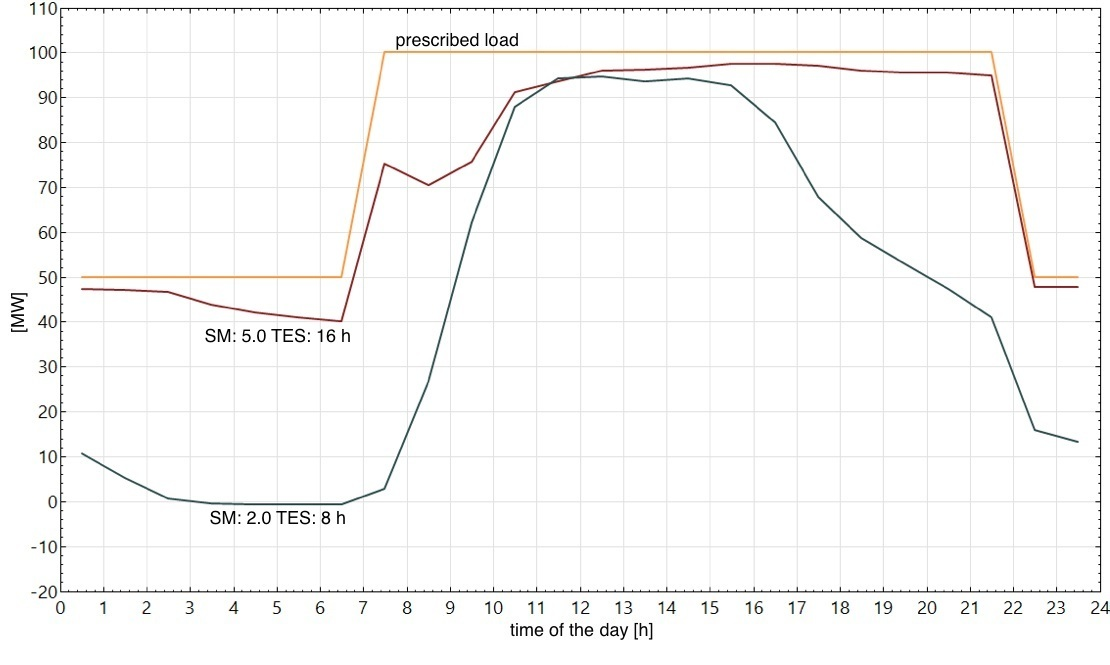
\includegraphics[width=0.8\linewidth]{FIG/PTC_annual_profil}
\caption[Annual average load profile of selected PTC power plant configurations.]{Annual average load profile of selected PTC power plant configurations.}\label{PTC_annual_profil}
\end{figure}
%The annual average load curve covering result of the selected simulated PTC configurations is shown in Figure~\ref{PTC_annual_profil}. It can be seen, that the PTC power plant using a SM of 5.0 and \SI{16}{h} of TES covers mostly any time of the year the prescribed load curve. But it is also obviously that power supply declines during the night from \SI{3}{am} on and is also decreasing in the morning hours at \SI{8}{am}. In comparison to that covers the PTC power plant using a SM of 2.0 and \SI{8}{h} of TES significantly less of the year the prescribed load curve. This simulated configuration of the PTC system starts declining the covering directly in the afternoon and standstill during the night from 3 to \SI{6}{am} during the whole year. All annual average load profile simulation results can be found in Appendix~\ref{all_load_profile}.

The load curve coverage of the selected simulated configurations is shown in Figure~\ref{PTC_annual_profil}. The plant using a SM of \num{5.0} and \SI{16}{h} of TES covers the prescribed load curve most of the year. Output declines during the night from \SI{3}{am} on and is also decreasing in the morning hours at \SI{8}{am}. The plant using a SM of \num{2.0} and \SI{8}{h} of TES has poorer coverage. In this configuration, output begins declining in the afternoon and drops entirely during the night from \num{3} to \SI{6}{am} throughout the year. All annual average load profile simulation results may be found in Appendix~\ref{all_load_profile}.

%Figure~\ref{PTC_winter_load} shows the load curve behavior of the selected PTC power plant configurations during the time of winter solstice, so the time with the shortest time of sunlight and the lowest angle of the incoming sunlight in Upington, SA. In the portrayed time line the DNI coming fro the whether file has a maximum of a about \SI{830}{\watt\per\square\metre} in peak times and there are also days with lower or almost no direct irradiance. 

Figure~\ref{PTC_winter_load} shows the load curve behaviour of the selected configurations around the northern solstice, that being the time with the fewest daylight hours and the lowest angle of incidence. During this period, maximum DNI is \SI{830}{\watt\per\square\metre} in peak times. There are also days with lower or almost no direct irradiance.

\begin{figure}[htbp]  
\centering
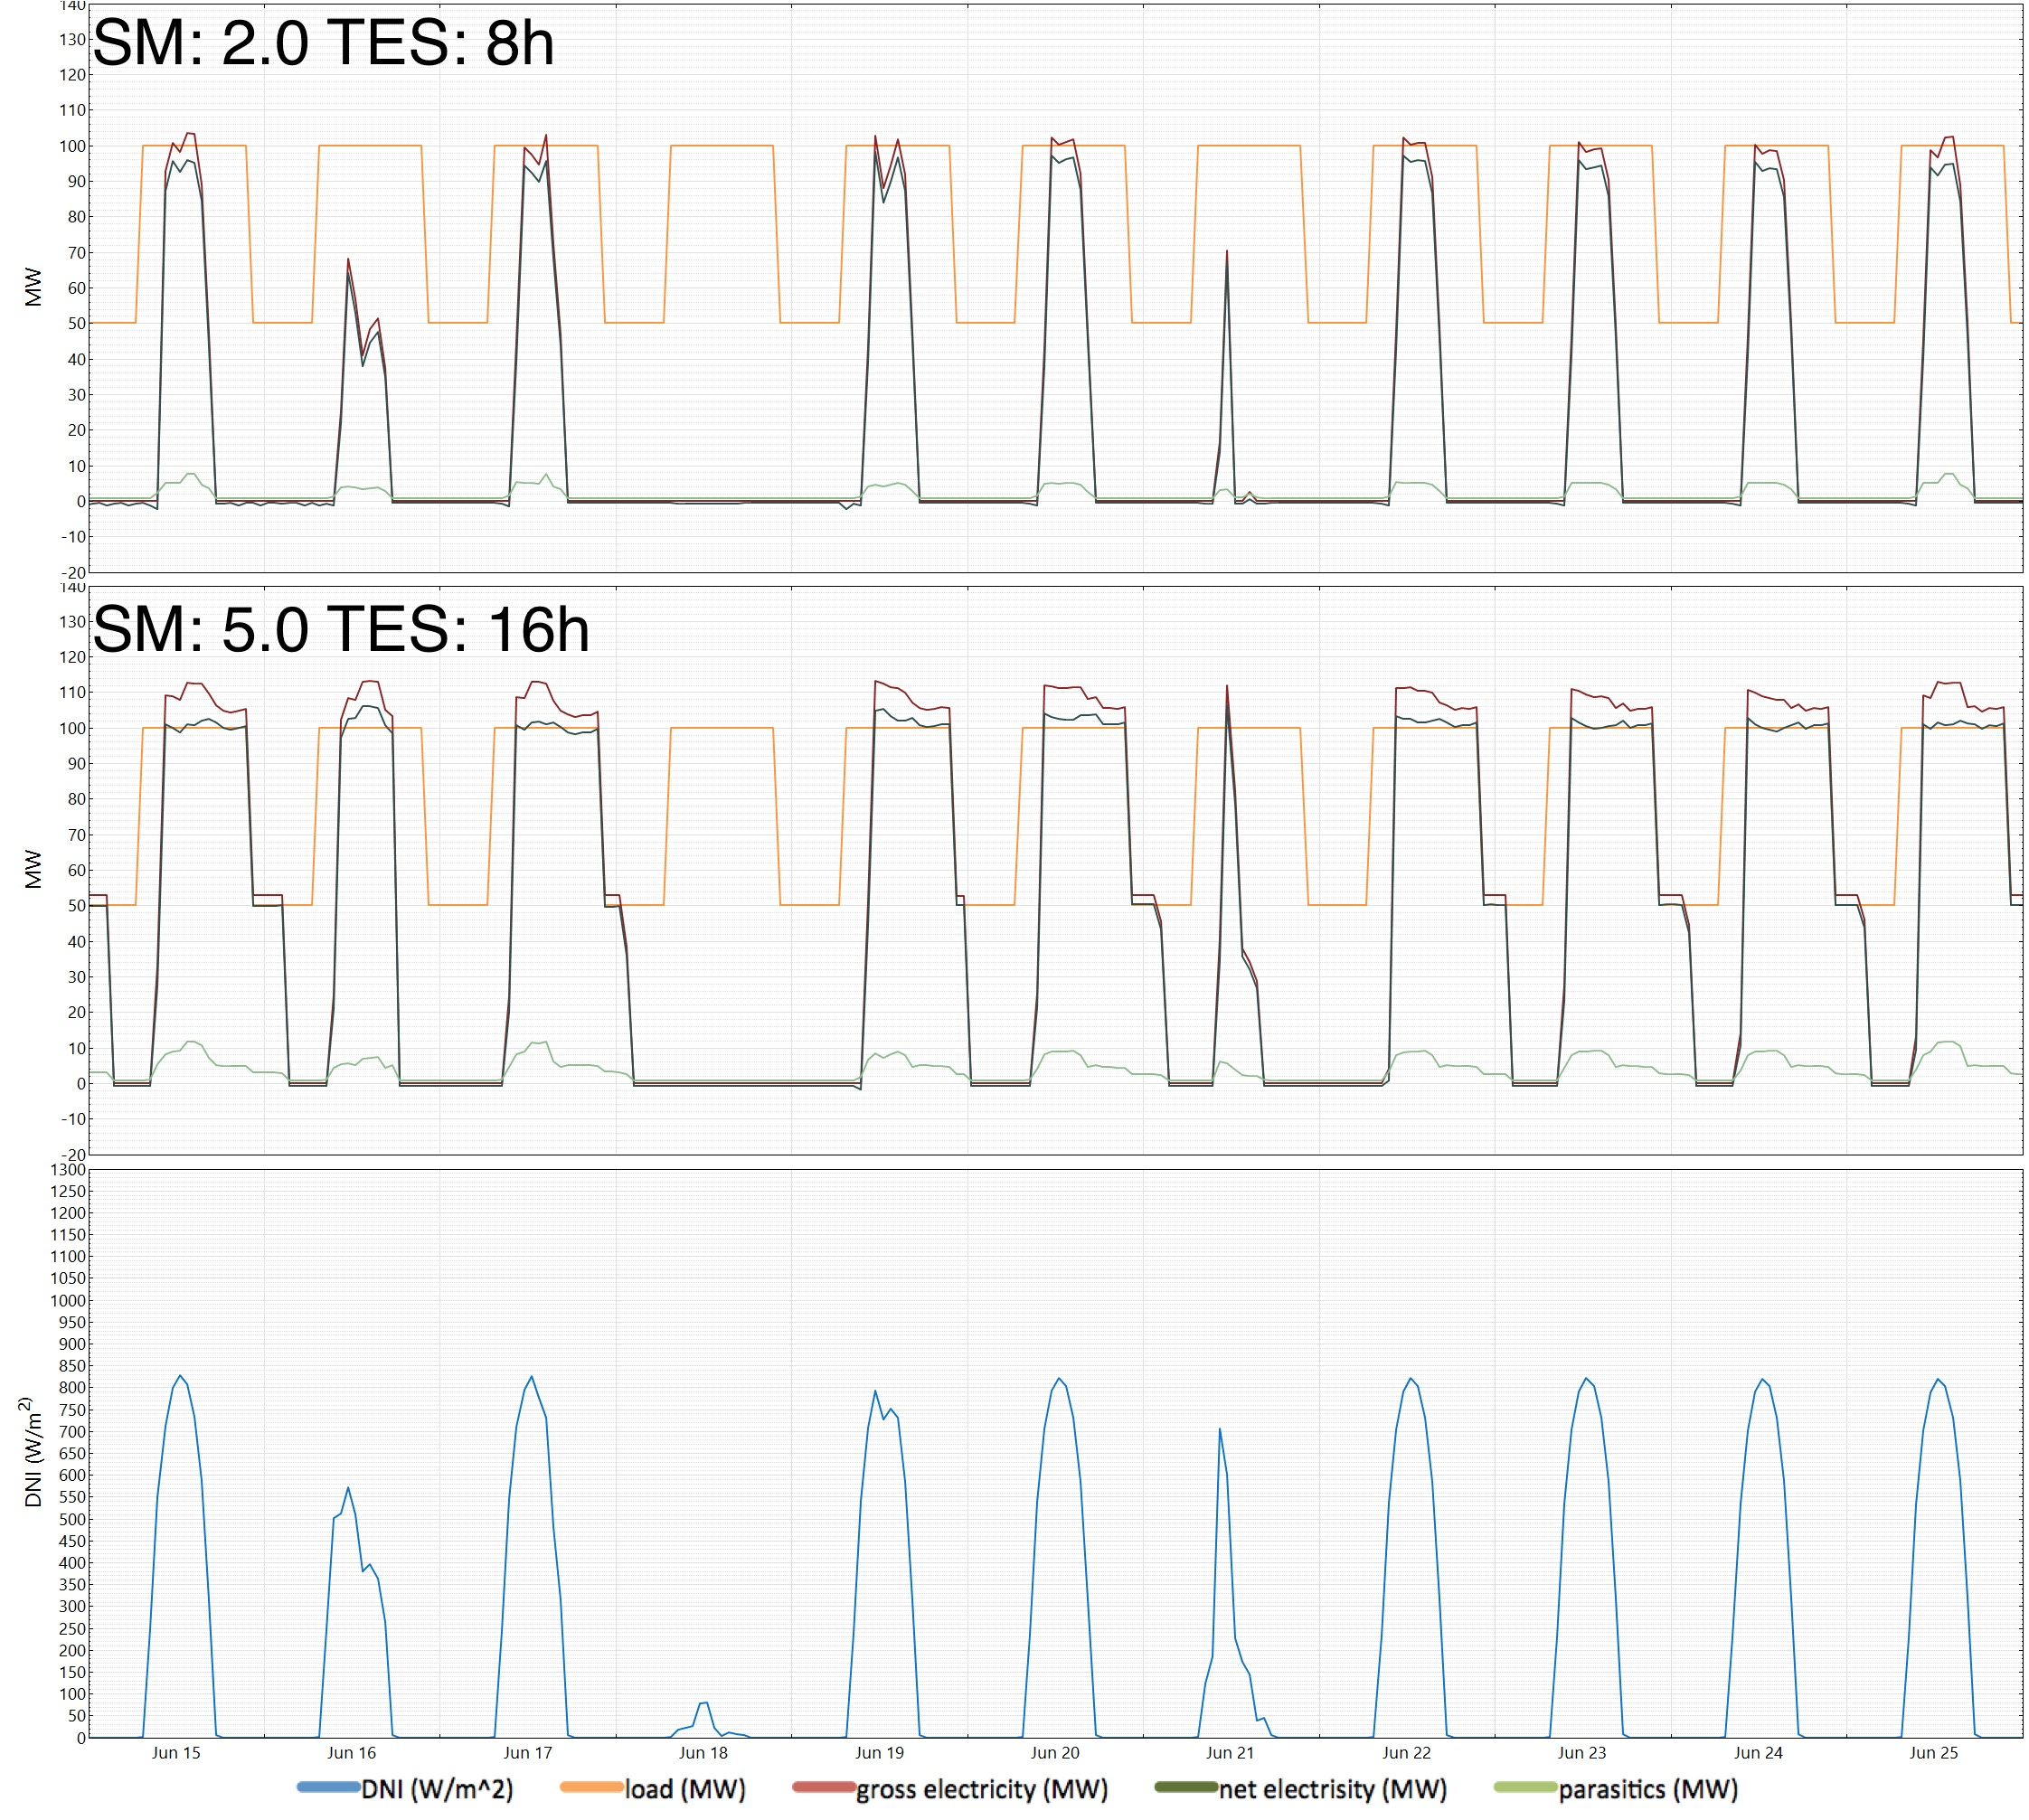
\includegraphics[width=1\linewidth]{FIG/PTC_winter_load}
\caption[PTC load profile around the northern solstice (15. June - 25. June).]{PTC load profile around the northern solstice (15. June - 25. June).}\label{PTC_winter_load}
\end{figure}
%The net electricity production of the PTC power plant with low configurations don't reach the prescribed load at any time in this portrayed time line. Therefore it is obviously that the solar field don't collect enough thermal energy during the day for filling up the storage to supply the steam turbines also by night. The power that is produced by the solar field goes at any time directly to the power generation and without direct sun irradiance the production is coming to standstill. The parasitic consumer has a peak load of about \SI{8}{MW} during these days in these configuration.

The net electricity production of the PTC plant with a small configuration does not cover the prescribed load at any point in this time-line. The solar field does not collect enough thermal energy during the day to charge the storage. All power converted by the solar field goes directly to electricity generation; without direct sun irradiance, generation stops entirely. Parasitic consumers cause a peak load of about \SI{8}{MW} during this period.

%In comparison to that is reaches the net electricity production of the PTC power plant with high configurations almost everyday the prescribed load for some hours. These configuration can also produce enough thermal energy by the solar field to fill up the storage to produce energy till after midnight. But also in that configuration is coming to standstill every night and rises first with the incoming direct irradiance again. In this configuration there is a peak load of about \SI{12}{MW} coming from the parasitic consumer. 

The plant with a large configuration can cover the prescribed load on almost any day, at least for a few hours. Such configurations can convert enough thermal energy from the solar field to continue generating until after midnight. Even this configuration drops out every night, rising only direct irradiance returns. In this configuration, parasitic loads are \SI{12}{MW}. 


%The overproduction of the net output depends on the gross output control and the variable parasitic consumers. The turbine output was preset for all PTC power plant simulation using the turbine output fraction of the TES dispatch control matrix which illustrated in Figure~\ref{PTC_turbineoutput} on Page~\pageref{PTC_turbineoutput}. So it was not possible to regulate the net output under variable external influences at any time. 

The overproduction of net output depends on gross output control and variable parasitic consumers. The turbine output was pre-set for all PTC simulations using the turbine output fraction of the TES dispatch control matrix, illustrated in Figure~\ref{PTC_turbineoutput} on page~\pageref{PTC_turbineoutput}. As a result, it was not possible to regulate the net output under variable external influences at any time.

%It is obviously that the performance of the PCT power plant isn't great at all during the winter solstice. Neither under high then low performance configurations. This leads mainly from the declining optical performance of the solar collector field under impact of lower sunlight angle during the winter months. This performance loss can mainly reduce to the cosine efficiency of the solar field. Figure~\ref{PTC_field_eff} gives an impression of the strong influence of the cosine efficiency on the total optical field efficiency of the simulated PTC power plants. It can be seen that the cosine effect reduces the total field efficiency by almost 50~\% during the midday in June. 

The performance of PTC power plants, at least in this simulation, is poor during northern solstice, irrespective of configuration. This is primarily a result of declining optical performance of the solar collector field under lower sunlight angle during the winter months. This performance loss can be attributed to the cosine efficiency of the solar field. Figure~\ref{PTC_field_eff} gives an impression of the influence of cosine efficiency on the total optical field efficiency of the simulated PTC power plants. The cosine effect reduces the total field efficiency by almost \SI{50\{\percent} at midday in June. 


\begin{figure}[!htbp]
        \centering                
        \begin{subfigure}[b]{0.5\textwidth}
                \centering
                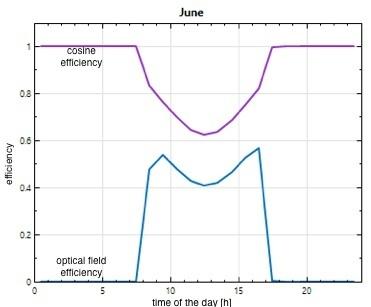
\includegraphics[width=1\textwidth]{FIG/PTC_field_eff_winter}
                \caption{Avarage influence of the cosine efficiency on the avarage total optical field efficiency in June.}\label{PTC_field_eff_winter}
        \end{subfigure}%
        ~
        \begin{subfigure}[b]{0.5\textwidth}
                \centering
                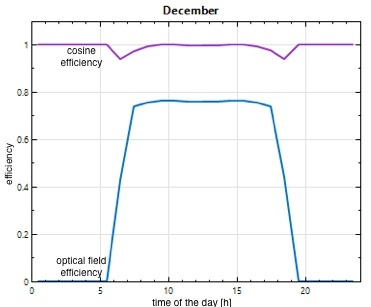
\includegraphics[width=1\textwidth]{FIG/PTC_field_eff_summer}
                \caption{Avarage influence of the cosine efficiency on the avarage total optical field efficiency in December.}\label{PTC_field_eff_summer}
        \end{subfigure}
        \caption[Influence of the cosine efficiency on average total optical field efficiency of a PTC power plant for different months of the year.]{Influence of the cosine efficiency on average total optical field efficiency of a PTC power plant for different months of the year.}\label{PTC_field_eff}
\end{figure}
%The loss in optical field performance by the cosine effect arise from the low angle of sunlight, therefor is the efficiency loss in the summer months through the cosine effect comparability low and has just an low effect in the morning and evening hours. 
%
%The load behavior of the two exemplary PTC power plants during the summer solstice is shown in Figure~\ref{PTC_summer_load}. It is obviously that the higher values of the DNI which reaches 1~\SI{150}{\watt\per\square\metre} in peak and the better field efficiency leads to a considerably higher covering of the prescribed load in both configurations. 

The loss in optical field performance by cosine effect arises from the low angle of sunlight, so the efficiency loss through the cosine effect is comparably low in summer, and the effect here is limited to morning and evening hours. 

%The load behavior of the two exemplary PTC power plants during the summer solstice is shown in Figure~\ref{PTC_summer_load}. It is obviously that the higher values of the DNI which reaches 1~\SI{150}{\watt\per\square\metre} in peak and the better field efficiency leads to a considerably higher covering of the prescribed load in both configurations. 

The load behaviour of the two example plants at southern solstice is shown in Figure~\ref{PTC_summer_load}. Values for DNI reach \SI{1150}{\watt\per\square\metre} at peak, and better field efficiency leads to a considerably higher coverage of the prescribed load in both configurations. 

\begin{figure}[htbp]  
\centering
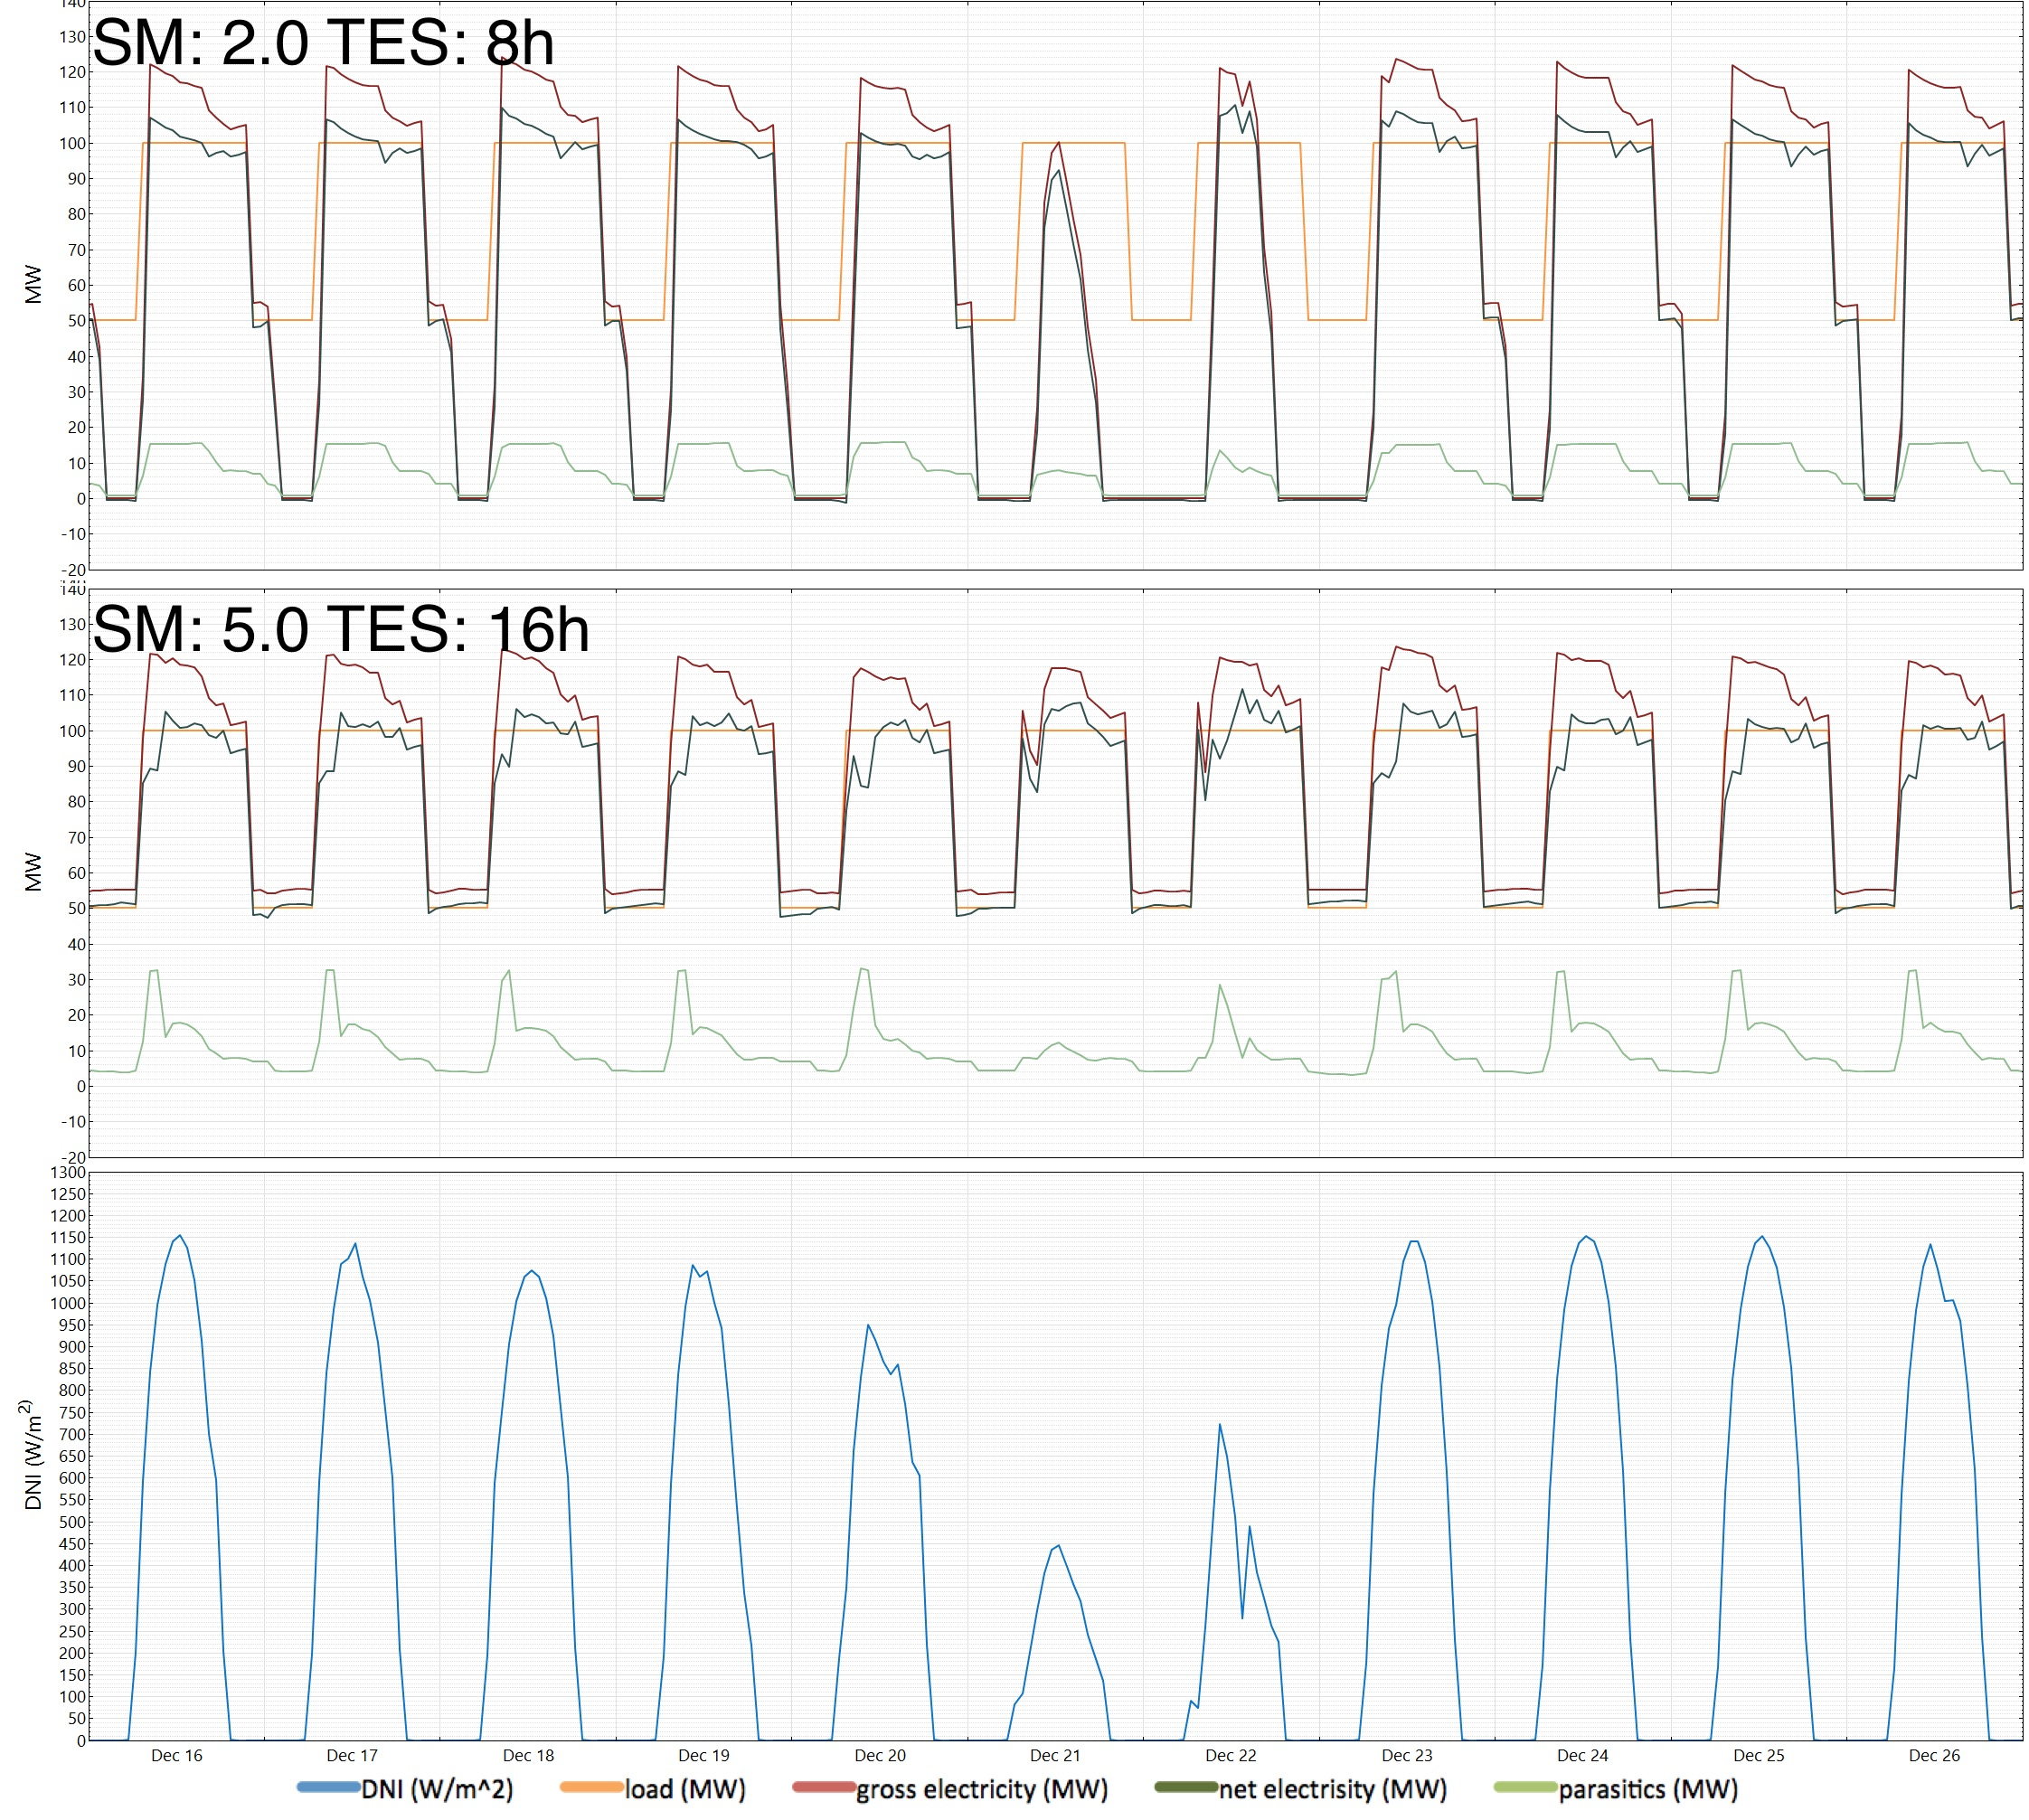
\includegraphics[width=1\linewidth]{FIG/PTC_summer_load}
\caption[PTC load profile during the time of summer solstice (16. December - 26. December).]{PTC load profile during the time of summer solstice (16. December - 26. December).}\label{PTC_summer_load}
\end{figure}
%The lower PTC configuration which is using a SM of 2.0 and \SI{8}{h} of TES can cover almost the full daytime load and a part of the night time load eith the net electricity production. But under this configuration the PTC power plant can't cover the prescribed load during the night at the best irradiance time of the year, therefrom is also the mentioned gap in production in the annual average load curve coming which was mentioned at the beginning of these section. The net electricity production over-scaled prescribed load at the beginning of the days which leads from the mentioned gross power output control. The parasitic consumers reaching a peak demand of \SI{15}{MW} in this configuration. 

The smaller PTC configuration using a SM of \num{2.0} and \SI{8}{h} of TES can cover almost the full daytime load and part of the night time load. However, the plant cannot cover the prescribed load at night even during times of highest irradiance. Parasitic loads peak at \SI{15}{MW}. 


%Figure~\ref{PTC_summer_load} shows also the load behavior of the PTC power plant with the highest simulated configuration, which doesn't stand still in this portrayed time span. The graph shows that the net out put is not constant at all. This is coming from the gross power output control and from the massive rises from the parasitic consumers, especially the solar field HTF pump. These pump needs to move a high volume of HTF through the HCEs. At a SM of 5.0 the solar field produce 5 times that much heat then the steam turbine actually needs at the design point. This over-scaling is necessary for the energy production in winter times during the night. Therefore the fractions of focused SCA's getting reduced when the generated energy filled up the storage completely and no more energy in demanded by the steam turbine. This is what  happens to the total parasitic consumption in the chart. The fractions of focused SCA's getting reduced so the power of solar field HTF pump is getting reduced as well. The peak of the parasitic consumers reaching a demand of about \SI{33}{MW} which makes about 27.5~\% of the gross turbine capacity.

Figure~\ref{PTC_summer_load} also shows the load behaviour of the PTC power plant with the highest simulated configuration, which does not drop out in this time span. The graph shows that the net out put is not constant at all. This is coming from the gross power output control and from the massive rises from the parasitic consumers, especially the solar field HTF pump. These pump needs to move a high volume of HTF through the HCEs. At a SM of 5.0 the solar field produce 5 times that much heat then the steam turbine actually needs at the design point. This over-scaling is necessary for the energy production in winter times during the night. Therefore the fractions of focused SCA's getting reduced when the generated energy filled up the storage completely and no more energy in demanded by the steam turbine. This is what  happens to the total parasitic consumption in the chart. The fractions of focused SCA's getting reduced so the power of solar field HTF pump is getting reduced as well. The peak of the parasitic consumers reaching a demand of about \SI{33}{MW} which makes about 27.5~\% of the gross turbine capacity.


\begin{figure}[!thbp]
        \centering   
        \begin{subfigure}[b]{0.65\textwidth}
                \centering
                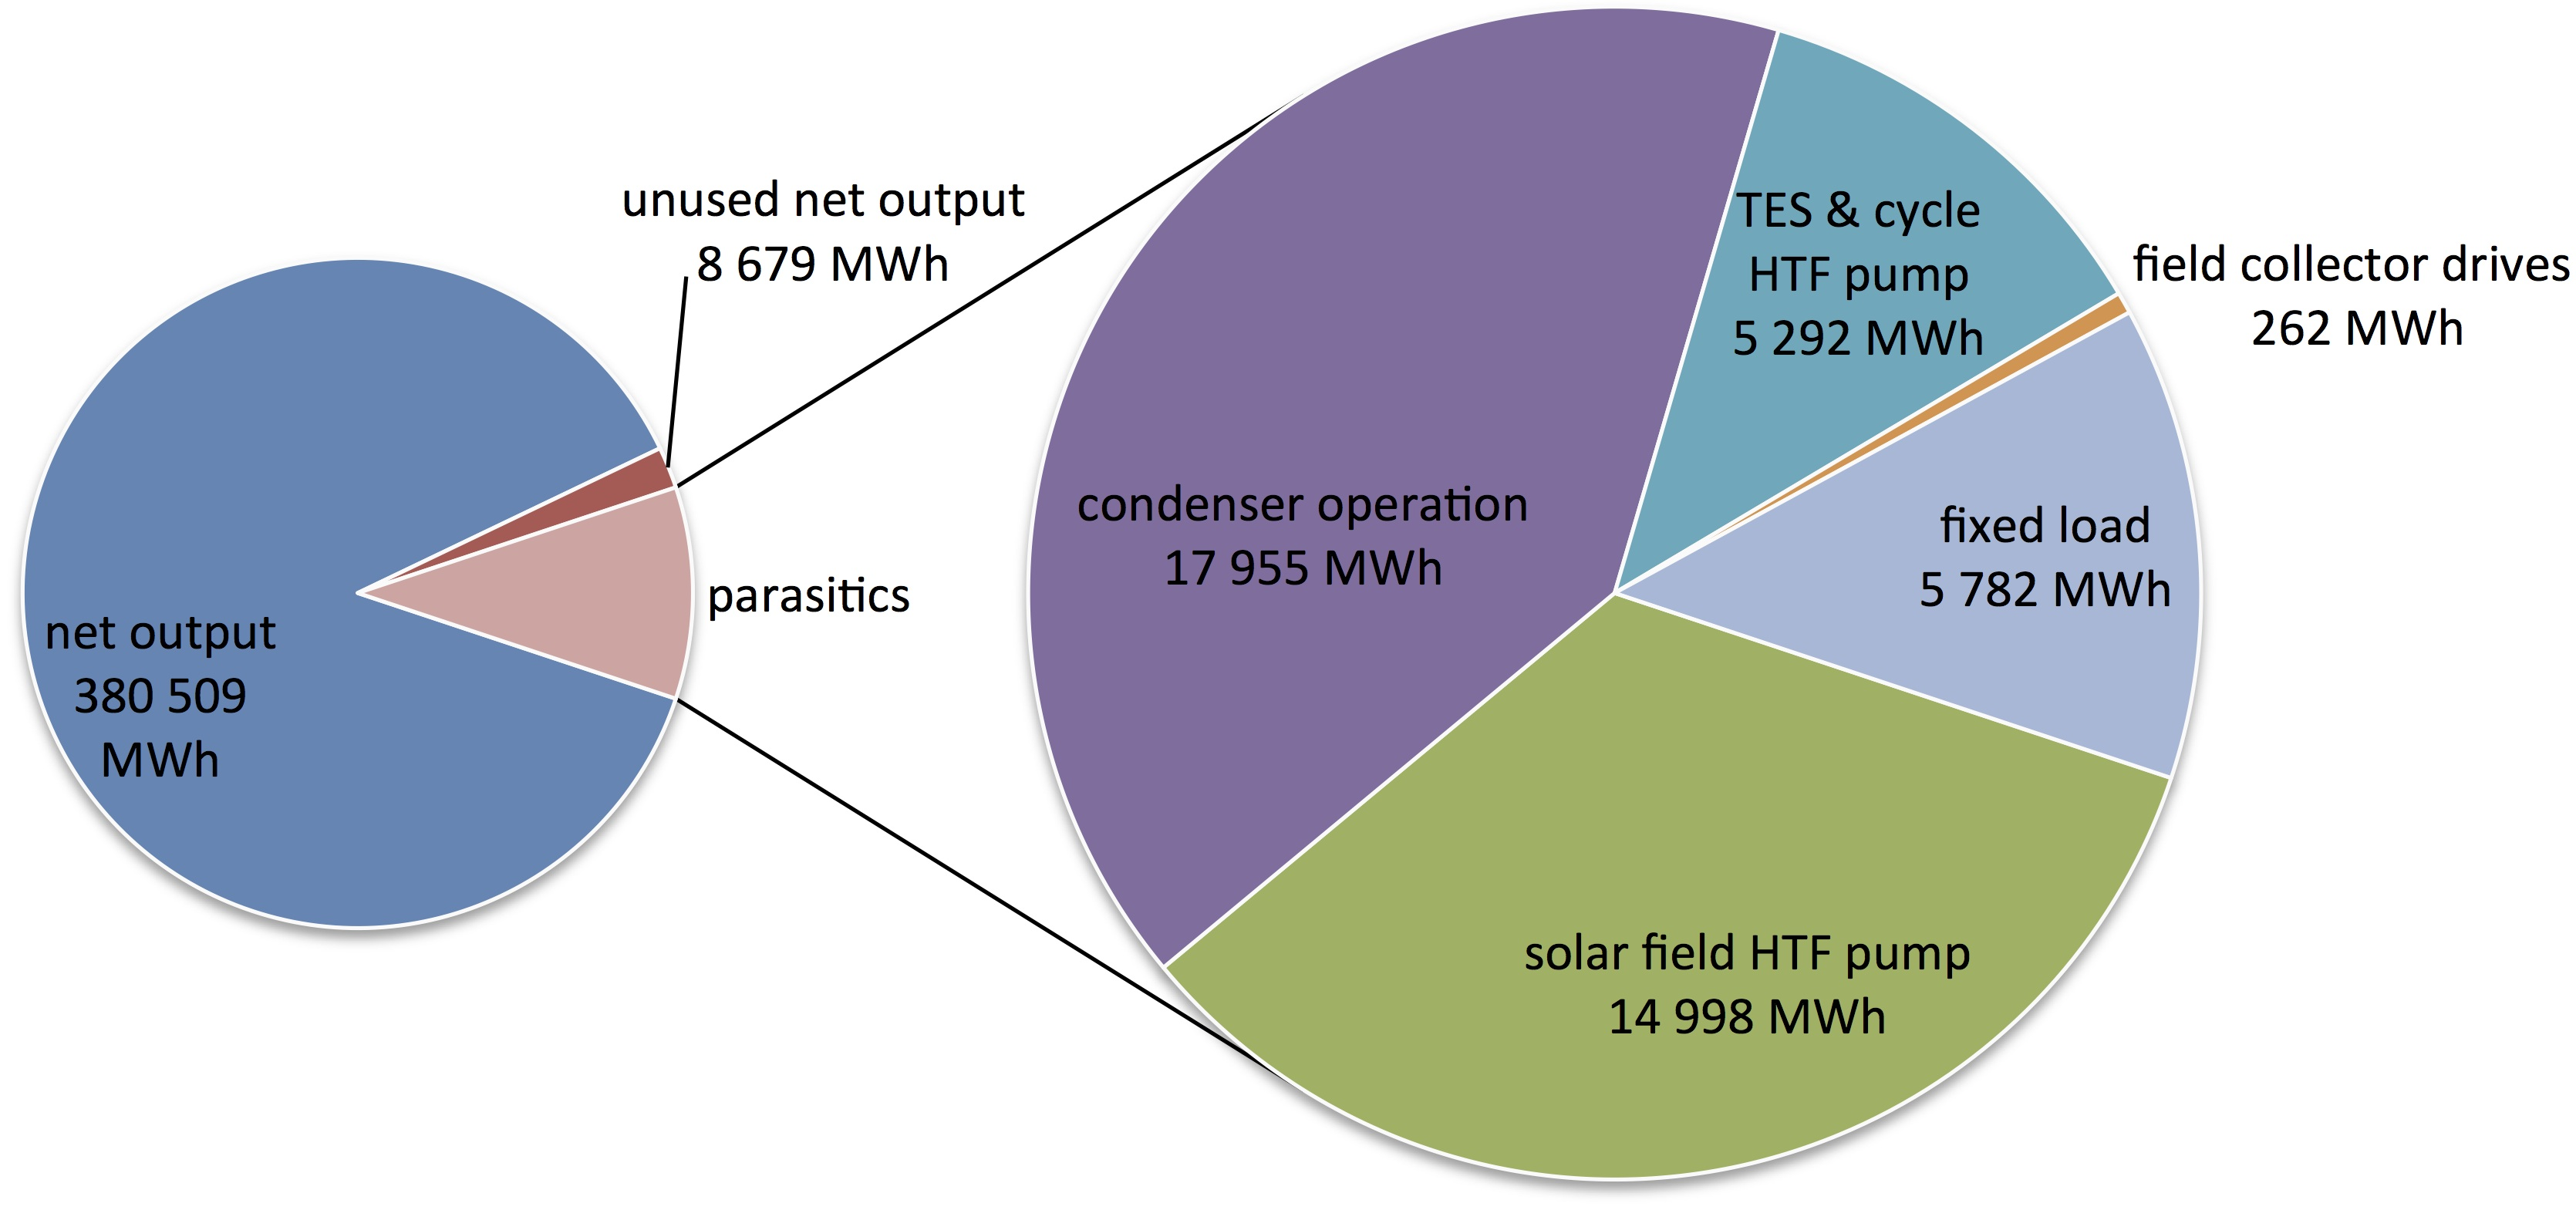
\includegraphics[width=1\textwidth]{FIG/PTC_parasitics_low}
                \caption{SM: 2.0 TES: 8 h}\label{PTC_parasitics_low}
        \end{subfigure}
\par\medskip % Linebreak              
        \begin{subfigure}[b]{0.65\textwidth}
                \centering
                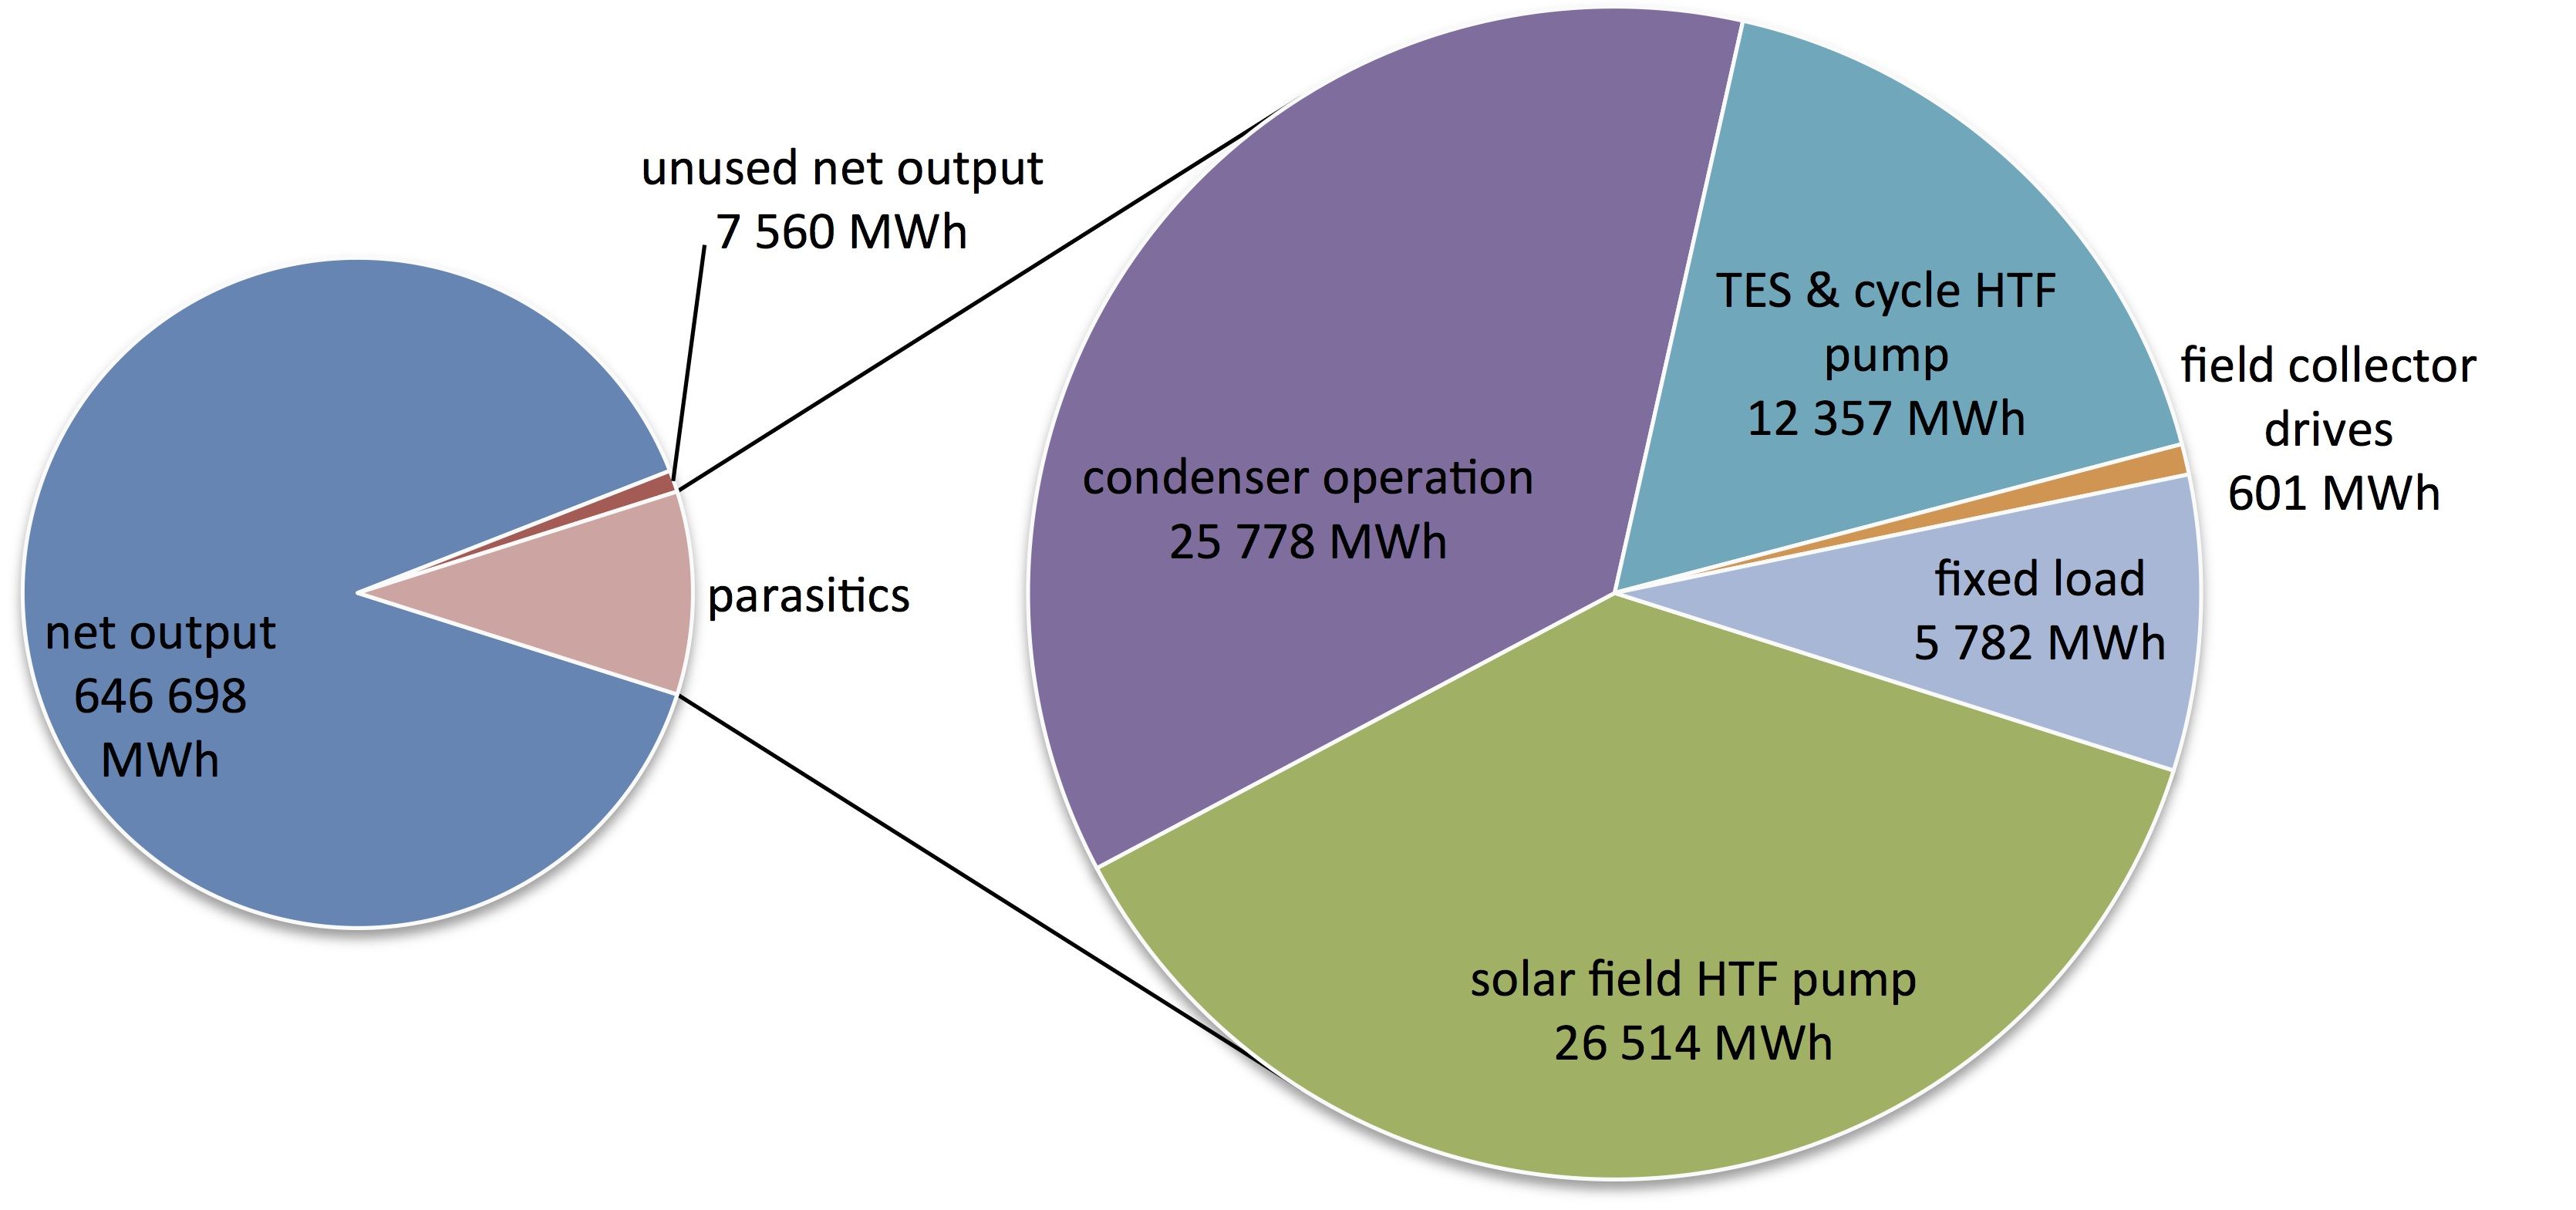
\includegraphics[width=1\textwidth]{FIG/PTC_parasitics_high}
                \caption{SM: 5.0 TES: 16 h}\label{PTC_parasitics_high}
        \end{subfigure}
        \caption[Share of annual gross energy output of selected PTC power plant configurations.]{Share of annual gross energy output of selected PTC power plant configurations.}\label{PTC_parasitics}
\end{figure}
The parasitic demand is composed from different electrical loads of the PTC power plant. Dominantly is the mentioned solar field HTF pump but also the condenser operation of the power cycle. Additionally are the parasitic consumption of the TES \& cycle HTF pump, the field collector drives and the fixed loads. Figure~\ref{PTC_parasitics} shows the share of the produced gross energy of the selected configurations for the simulated year. About 10~\% of the annual gross energy production is going to the parasitic consumers. Therefrom goes about one-third respectively to the condenser operation and the solar field HTF pump. The reaming parasitic load is shared by the TES \& cycle HTF pump and the fixed loads. The share of the field collector drives to the parasitic loads is below 1~\% in any case.

Figure~\ref{PTC_parasitics_low} names the total net output for covering the prescribed load at about \SI{380.51}{GWh} for the PTC power plant with a SM of 2.0 and \SI{8}{h} of TES. The total sum of the annual prescribed load is \SI{711.75}{GWh}. Therefrom results a covering of 53.5~\% of the PTC power plant with the lowest configurations. The annual net output result of the highest simulated PTC configuration can be found in Figure~\ref{PTC_parasitics_high} and is about \SI{646.70}{GWh} which results in a load covering from about 90.9~\% over the year of the prescribed load. 

The remaining load covering results of all simulated PTC power plants can be found in Figure~\ref{PTC_LCCF}. The chart shows that at a SM of 2 all simulated TES variations reaching a load curve covering of 53.4~\%. It can be noteced that the growing rate of the covering is declining with the rising SM. The growing rate from the SM 2.0 to 2.5 is between 10.9~\% and 14.9~\% while it is from the SM 4.5 to 5.0 just between 1~\% and 2~\%. Also there is no noticeable gain between using 12, 14 or \SI{16}{h} of TES. The difference is at highest 0.7~\%. 

\begin{figure}[bhtp]  
\centering
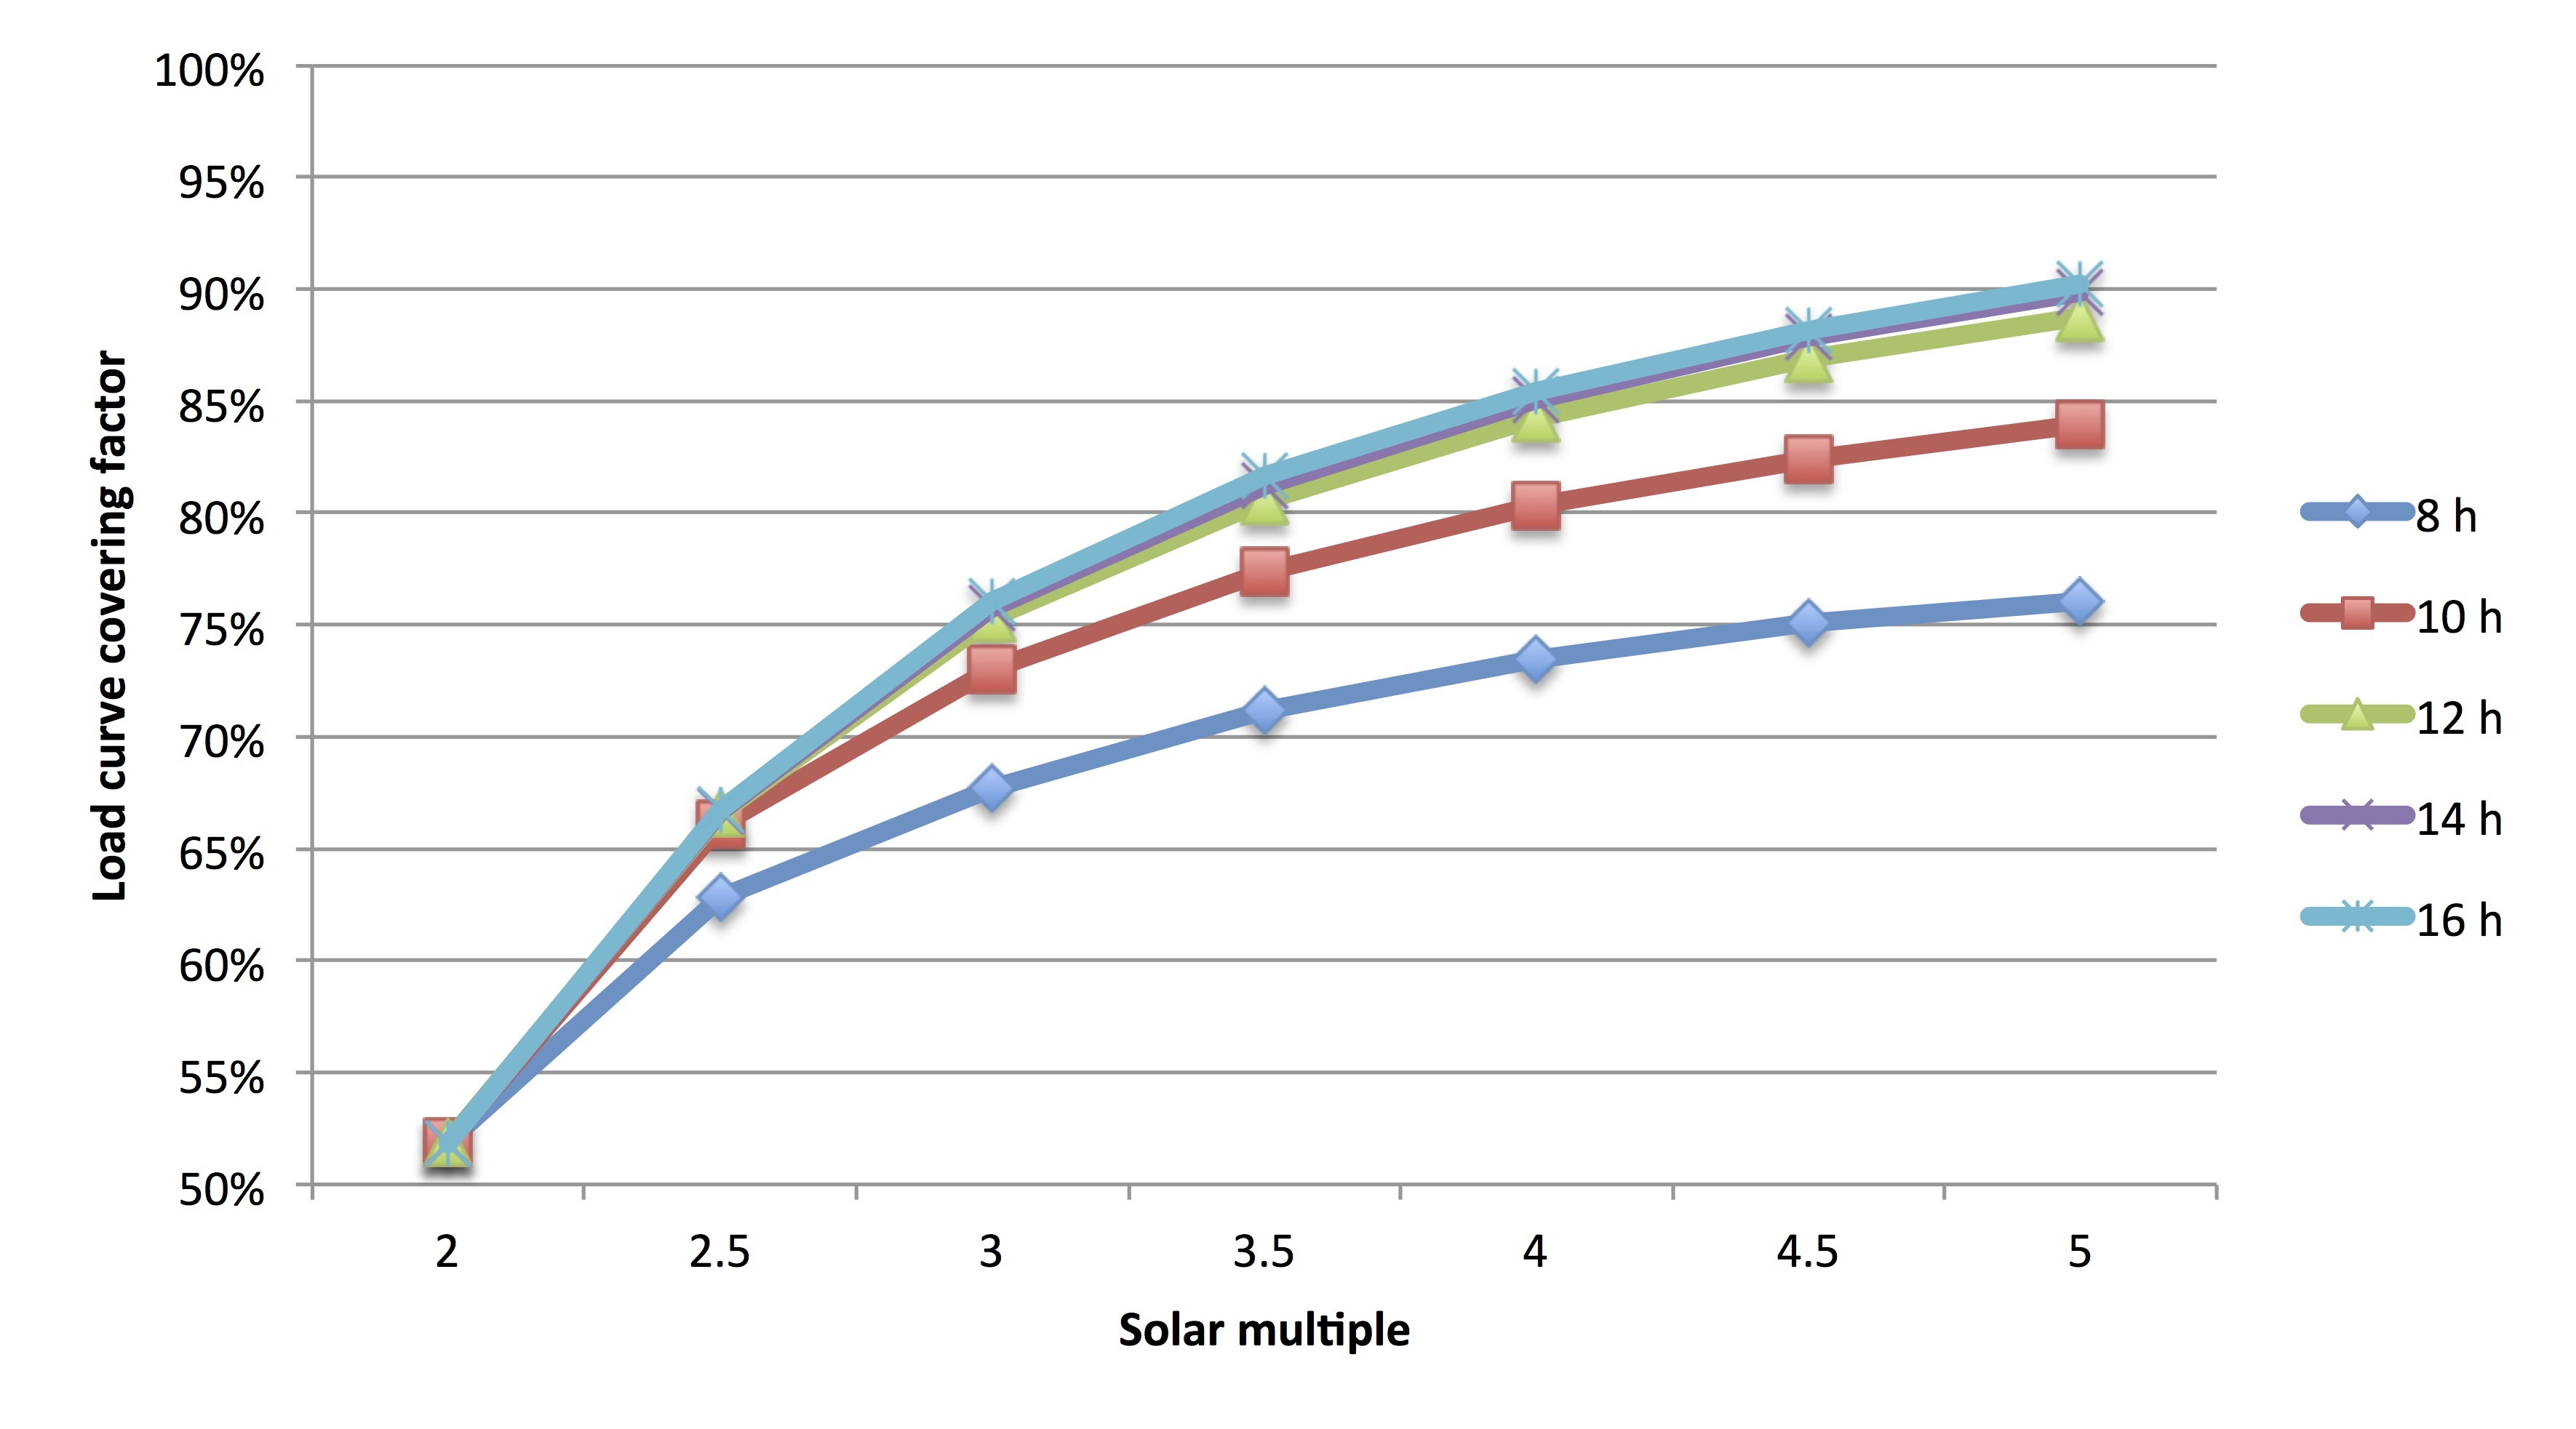
\includegraphics[width=1\linewidth]{FIG/PTC_LCCF}
\caption[Load curve covering result of simulated PTC systems.]{Load curve covering result of simulated PTC systems.}\label{PTC_LCCF}
\end{figure}
The target of 90~\% load covering is just reached by a SM of 5.0 and more then \SI{12}{h} of TES and it can be noted that it seams to be really elaborate for reaching that high value of annual covering using a PTC plant. 70~\% load covering was reached at all simulated PTC configurations. While 80~\% load covering was reached by all configurations besides the \SI{8}{h} of TES.
\subsubsection{Levelized costs of electricity}
For the calculated LCOE the finacial input parameter in Table~\ref{tbl: PTCFinance} and a simplified method which is documented in Appendix~\ref{ChapterLCOE} on Page \pageref{ChapterLCOE} was used. These results of the LCOE claculation for the simulated PTC configurations can be seen in Figure~\ref{PTC_LCOE}. 

The lowest LCOE result of the simulated PTC power plants is \SI{144.91}{USD/MWh} at a SM of 3.0 and \SI{10}{h} of TES. The \SI{8}{h} TES at a SM of 2.5 has marginal higher result of (\SI{145.17}{USD/MWh}). The highest LCOE result of \SI{202.95}{USD/MWh} was reached at a SM of 2.0 and \SI{16}{h} of TES. 

Depending from almost identical load curve covering is the behavior of LCOE results of the simulated TES variations 12, 14 and \SI{16}{h} almost identical. The difference in the height of the charts results from the higher investment cost of the larger storage configuration.

\begin{figure}[htbp]  
\centering
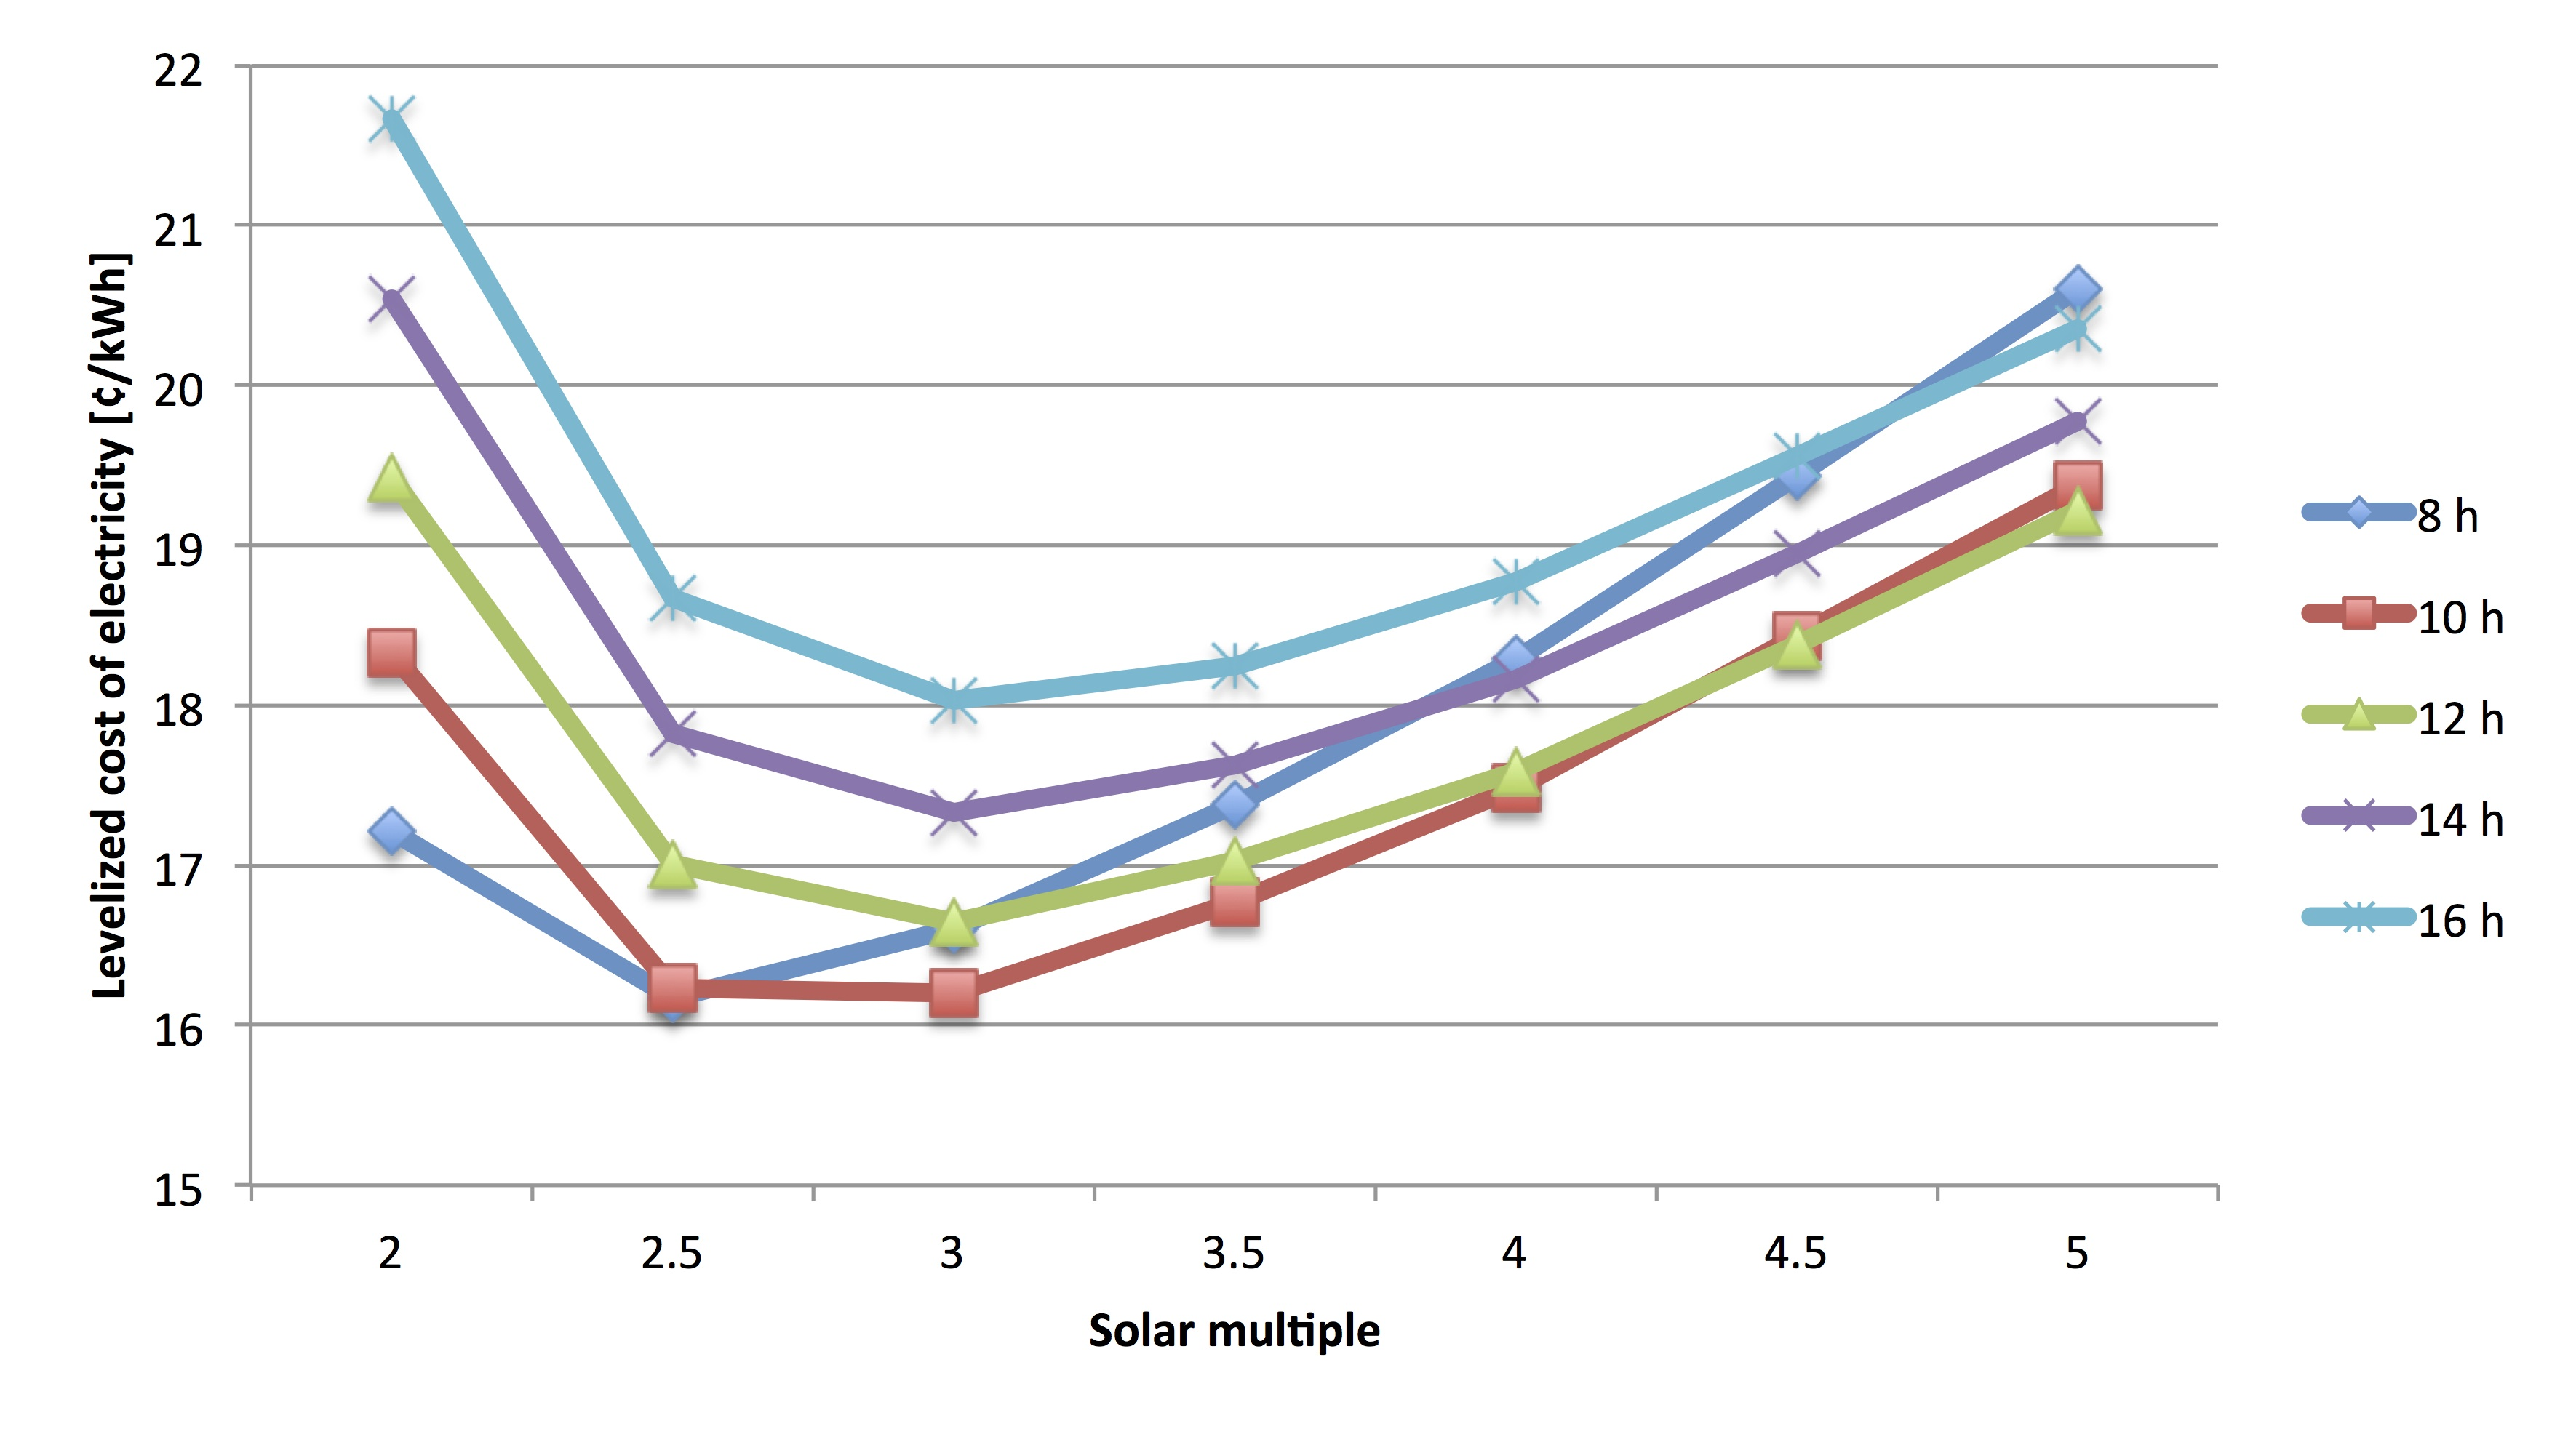
\includegraphics[width=1\linewidth]{FIG/PTC_LCOE}
\caption[LCOE calculation results for PTC simulation.]{LCOE calculation results for PTC simulation.}\label{PTC_LCOE}
\end{figure}

When comprising the load curve covering results and the LCOE calculation results of the simulated PTC power plants, the lowest LCOE for reaching the target of 90~\% load curve covering is \SI{167.45}{USD/MWh} at a SM of 5.0 and \SI{12}{h} of TES. 

For reaching a covering of 80~\% of the load curve the PTC configuration with a SM of 3.5 and \SI{12}{h} of TES has the lowest LCOE with \SI{151.84}{USD/MWh}. The lowest LCOE for reaching 70~\% of the prescribed load curve is \SI{144.91}{USD/MWh} at a SM of 3.0 and \SI{10}{h} of TES.
\pagebreak